%% ============================================================
%%  Bakalářská práce — ČVUT FEL
%%  Šablona: CTUstyle3 / LaTeX (babel + lmodern)
%%
%%  Kompilace:  pdflatex main.tex
%%              (2× pro správné reference a TOC)
%% ============================================================

\documentclass[
  a4paper,          % formát papíru A4
  11pt,             % velikost základního písma
  oneside,          % jednostranná sazba (bez prázdných stránek mezi kapitolami)
  openany           % kapitoly začínají na libovolné straně
]{report}

%% ── Kódování a jazyk ─────────────────────────────────────────
\usepackage[T1]{fontenc}
\usepackage[utf8]{inputenc}
\usepackage[czech]{babel}

%% ── Písmo: Latin Modern (požadavek ČVUT) ─────────────────────
\usepackage{lmodern}

%% ── Geometrie stránky ────────────────────────────────────────
%% Vnitřní okraj 30 mm (pro pevnou vazbu), ostatní ~25 mm
\usepackage[
  a4paper,
  inner=30mm,
  outer=20mm,
  top=25mm,
  bottom=25mm,
  headheight=15pt
]{geometry}

%% ── Barva CTU blue ───────────────────────────────────────────
\usepackage[dvipsnames]{xcolor}
\definecolor{CTUblue}{HTML}{0065BD}   % Pantone 300 C

%% ── Formátování nadpisů — modré dle CTUstyle ─────────────────
\usepackage{titlesec}
\titleformat{\chapter}[display]
  {\normalfont\huge\bfseries\color{CTUblue}}
  {\chaptertitlename\ \thechapter}{20pt}{\Huge}
\titleformat{\section}
  {\normalfont\Large\bfseries\color{CTUblue}}
  {\thesection}{1em}{}
\titleformat{\subsection}
  {\normalfont\large\bfseries\color{CTUblue!80!black}}
  {\thesubsection}{1em}{}
\titleformat{\subsubsection}
  {\normalfont\normalsize\bfseries}
  {\thesubsubsection}{1em}{}

%% ── Řádkování ────────────────────────────────────────────────
\usepackage{setspace}
\onehalfspacing      % 1,5-násobné řádkování (obvyklé pro závěrečné práce)

%% ── Kolontituly ──────────────────────────────────────────────
%% V záhlaví: číslo + název kapitoly | V patičce: číslo stránky u vnějšího okraje
\usepackage{fancyhdr}
\pagestyle{fancy}
\fancyhf{}
\fancyhead[LE,RO]{\small\leftmark}   % sudá vlevo / lichá vpravo: název kapitoly
\fancyfoot[LE,RO]{\thepage}          % číslo stránky u vnějšího okraje
\renewcommand{\headrulewidth}{0.4pt}

%% ── Obrázky a tabulky ────────────────────────────────────────
\usepackage{graphicx}
\graphicspath{{images/}{images/screenshots/}}
\usepackage{pdfpages}    % vkládání zadání jako PDF
\usepackage{float}
\usepackage{amssymb}  % \checkmark
\usepackage{booktabs}
\usepackage{tabularx}
\usepackage{caption}
\captionsetup{font=small, labelfont=bf}

%% ── Seznamy ──────────────────────────────────────────────────
\usepackage{enumitem}
\setlist{noitemsep, topsep=4pt}

%% ── Hypertextové odkazy (PDF bookmarks) ──────────────────────
\usepackage[
  colorlinks=true,
  linkcolor=CTUblue,
  citecolor=CTUblue,
  urlcolor=CTUblue,
  pdftitle={Software pro podporu digitalizace schvalovacího procesu v malé firmě},
  pdfauthor={Artem Arsenyev},
  pdfsubject={Bakalářská práce, ČVUT FEL}
]{hyperref}

%% ── Zdrojové kódy ────────────────────────────────────────────
\usepackage{listings}
\lstset{
  basicstyle=\ttfamily\small,
  breaklines=true,
  frame=single,
  numbers=left,
  numberstyle=\tiny\color{gray},
  commentstyle=\color{gray},
  keywordstyle=\color{CTUblue}\bfseries
}

%% ── Misc ─────────────────────────────────────────────────────
\usepackage{microtype}   % lepší sazba textu
\usepackage{csquotes}    % české uvozovky pomocí \enquote{}
\usepackage{url}

%% ============================================================
%%  METADATA — DOPLŇTE SVÉ ÚDAJE
%% ============================================================
\newcommand{\ThesisTitle}{Software pro podporu digitalizace schvalovacího procesu v malé firmě}
\newcommand{\ThesisTitleEN}{Software to support the digitalization of the approval process in a small business company}
\newcommand{\ThesisAuthor}{Artem Arsenyev}
\newcommand{\ThesisSupervisor}{Ing. Martin Dobiáš, Ph.D.}
\newcommand{\ThesisFaculty}{Fakulta elektrotechnická}
\newcommand{\ThesisDepartment}{Katedra počítačů}
\newcommand{\ThesisDate}{Květen 2026}               %% <-- DOPLŇTE měsíc

%% ============================================================
%%  ZAČÁTEK DOKUMENTU
%% ============================================================
\begin{document}

%% ── Titulní strana ───────────────────────────────────────────
\begin{titlepage}
  \thispagestyle{empty}
  \begin{center}
    \vspace*{1cm}

    %% Logo ČVUT
    
\includegraphics[width=4cm]{LogoCVUT.pdf}\\[1cm]

    {\Large\textbf{České vysoké učení technické v Praze}}\\[0.3cm]
    {\large\ThesisFaculty}\\[0.1cm]
    {\large\ThesisDepartment}\\[2.5cm]

    {\huge\bfseries\color{CTUblue}\ThesisTitle}\\[0.5cm]
    {\large\ThesisTitleEN}\\[2.5cm]

    {\large Bakalářská práce}\\[2cm]

    \begin{flushleft}
      \textbf{Autor:} \ThesisAuthor\\[0.3cm]
      \textbf{Vedoucí práce:} \ThesisSupervisor\\[0.3cm]
      \textbf{Datum:} \ThesisDate
    \end{flushleft}
  \end{center}
\end{titlepage}

%% ── Zadání bakalářské práce ─────────────────────────────────
%% PDF soubor zadani.pdf musí být v adresáři thesis/
\IfFileExists{zadani.pdf}{%
  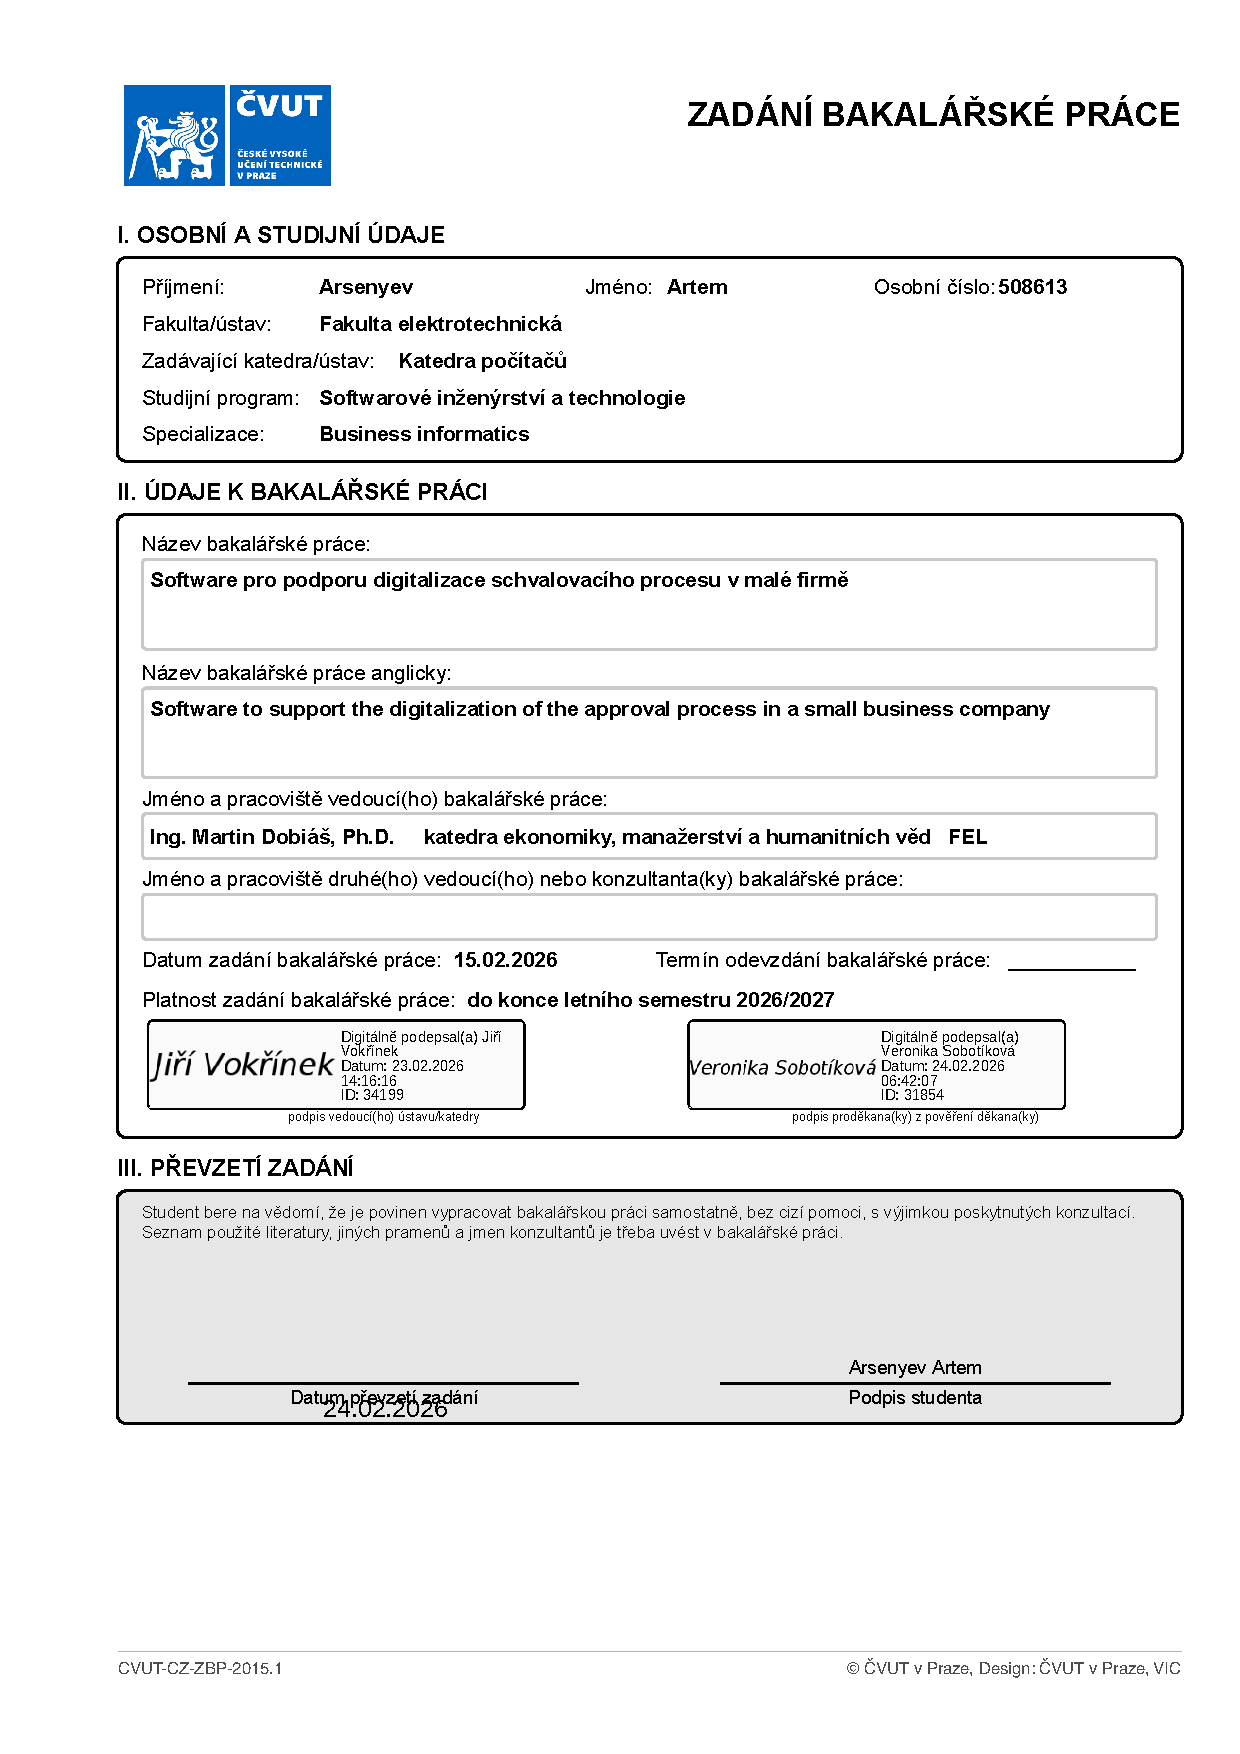
\includepdf[pages=1-2,pagecommand={\thispagestyle{empty}}]{zadani.pdf}%
}{%
  \cleardoublepage%
}

\cleardoublepage

%% ── Římské číslování pro úvodní část (Prohlášení, Poděkování, Abstrakt, TOC) ──
\pagenumbering{roman}
\setcounter{page}{1}

%% ── Poděkování ───────────────────────────────────────────────
\chapter*{Poděkování}
\addcontentsline{toc}{chapter}{Poděkování}
\thispagestyle{plain}

Rád bych poděkoval vedoucímu práce \ThesisSupervisor{} za odborné vedení a cenné rady
při zpracování této bakalářské práce. Dále děkuji společnosti Medicton Group za poskytnutí
interních podkladů a umožnění analýzy jejich procesů.

\cleardoublepage

%% ── Prohlášení ───────────────────────────────────────────────
\chapter*{Prohlášení}
\addcontentsline{toc}{chapter}{Prohlášení}
\thispagestyle{plain}

\noindent Já, níže podepsaný

\vspace{0.5cm}
\noindent\begin{tabular}{@{}p{6cm}l@{}}
Příjmení, jméno studenta: & Arsenyev Artem \\
Osobní číslo:             & 508613 \\
Název programu:           & Softwarové inženýrství a technologie \\
\end{tabular}

\vspace{0.8cm}
\noindent prohlašuji, že jsem bakalářskou práci s~názvem

\vspace{0.5cm}
\noindent\textbf{Software pro podporu digitalizace schvalovacího procesu v~malé firmě}

\vspace{0.5cm}
\noindent vypracoval samostatně a~uvedl veškeré použité informační zdroje v~souladu s~Metodickým pokynem o~dodržování etických principů při přípravě vysokoškolských závěrečných prací a~Rámcovými pravidly používání umělé inteligence na ČVUT pro studijní a~pedagogické účely v~Bc a~NM studiu.

\vspace{0.5cm}
\noindent Prohlašuji, že jsem v~průběhu příprav a~psaní závěrečné práce použil nástroje umělé inteligence. Vygenerovaný obsah jsem ověřil. Stvrzuji, že jsem si vědom, že za obsah závěrečné práce plně zodpovídám.

\vspace{2cm}
\noindent V~Praze dne 20.\,05.\,2026 \hfill Artem Arsenyev\\[0.2cm]
\hspace*{\fill} \dotfill\hspace{4cm}\\
\hspace*{\fill} podpis studenta\hspace{3cm}

\cleardoublepage

%% ── Abstrakt česky ───────────────────────────────────────────
\chapter*{Abstrakt}
\addcontentsline{toc}{chapter}{Abstrakt}
\thispagestyle{plain}

%% TODO: Napište abstrakt (cca 150–250 slov)
Tato bakalářská práce se zabývá analýzou a implementací softwarového řešení pro podporu
digitalizace schvalovacího procesu v malé obchodní společnosti. Práce vychází z reálného
prostředí firmy Medicton Group, která v oblasti zdravotnické techniky využívá sdílené tabulky
pro řízení interních nákupů a předávání účetních dokladů ke zpracování. Cílem práce je
navrhnout a implementovat online systém, který tyto procesy standardizuje, automatizuje
a zajistí auditní stopu rozhodnutí.

V analytické části je popsána organizační struktura společnosti, používané informační systémy
a aktuální podoba AS-IS procesů. Dále jsou analyzována existující softwarová řešení na trhu.
Na základě analýzy je navržen cílový TO-BE model schvalovacích workflow a datová architektura
systému. Implementační část popisuje technické řešení postavené na technologiích Spring Boot,
Spring Security, PostgreSQL a Thymeleaf, nasazené v cloudovém prostředí Railway.

\vspace{0.5cm}
\noindent\textbf{Klíčová slova:} digitalizace, schvalovací proces, workflow, Spring Boot,
PostgreSQL, bakalářská práce

\cleardoublepage

%% ── Abstract in English ──────────────────────────────────────
\chapter*{Abstract}
\addcontentsline{toc}{chapter}{Abstract}
\thispagestyle{plain}

%% TODO: Translate your abstract to English
This bachelor's thesis deals with the analysis and implementation of a software solution
to support the digitalization of the approval process in a small business company.
The work is based on the real environment of Medicton Group, a company in the medical
equipment sector that uses shared spreadsheets for managing internal purchases and
passing accounting documents for processing. The goal of the thesis is to design and
implement an online system that standardizes and automates these processes while providing
a full audit trail of decisions.

The analytical part describes the company's organizational structure, the information systems
in use, and the current AS-IS process model. Existing software solutions on the market are
also analyzed. Based on this analysis, a target TO-BE model of approval workflows and the
system's data architecture are proposed. The implementation section describes the technical
solution built on Spring Boot, Spring Security, PostgreSQL, and Thymeleaf, deployed in
the Railway cloud environment.

\vspace{0.5cm}
\noindent\textbf{Keywords:} digitalization, approval process, workflow, Spring Boot,
PostgreSQL, bachelor's thesis

\cleardoublepage


%% ── Obsah (Table of Contents) ────────────────────────────────
\tableofcontents
\cleardoublepage

%% ── Seznam obrázků ───────────────────────────────────────────
\listoffigures
\addcontentsline{toc}{chapter}{Seznam obrázků}
\cleardoublepage

%% ── Seznam tabulek ───────────────────────────────────────────
\listoftables
\addcontentsline{toc}{chapter}{Seznam tabulek}
\cleardoublepage

%% ── Přechod na arabské číslování od kapitoly 1 (Úvod) ─────────
\pagenumbering{arabic}
\setcounter{page}{1}

%% ============================================================
%%  HLAVNÍ TEXT PRÁCE
%% ============================================================

%% ============================================================
\chapter{Úvod}
%% ============================================================

V posledních letech se digitalizace podnikových procesů stala jedním z hlavních nástrojů zvyšování efektivity řízení organizací. Moderní informační systémy umožňují automatizovat řadu administrativních, evidenčních i rozhodovacích činností, čímž přispívají k větší přehlednosti procesů, rychlejšímu sdílení informací, lepší kontrole nad daty a omezení chyb způsobených manuálním zpracováním. Přesto však v mnoha menších společnostech existují procesy, které zůstávají pouze částečně digitalizované nebo jsou podporovány jen pomocí jednoduchých nástrojů, jako jsou sdílené tabulky, e-mailová komunikace nebo neformální interní dohody. Jednou z takových oblastí bývá schvalování interních požadavků a předávání účetních dokladů ke zpracování.

Předmětem této bakalářské práce je analýza a návrh softwarového řešení podporujícího digitalizaci schvalovacího procesu v malé společnosti. Práce vychází z reálného prostředí firmy působící v oblasti prodeje zdravotnické techniky, servisních služeb a pravidelných kontrol zařízení. Zkoumaná společnost využívá několik informačních systémů pro podporu obchodních, servisních a účetních činností, avšak některé interní podpůrné procesy stále probíhají převážně manuálně. Typickým příkladem je schvalování nákupů a výdajů nebo předkládání účetních dokladů k zaúčtování a proplacení, které je v současnosti řešeno prostřednictvím sdílených tabulek, ukládání dokumentů do SharePointu a následné komunikace mezi zaměstnanci a účetním oddělením. Tato výchozí situace odpovídá zadání práce, podle něhož je nutné nejprve seznámit se s organizačním uspořádáním firmy, aktuálním stavem oběhu dokumentů a schvalovacího procesu, a následně navrhnout i implementovat vhodné online softwarové řešení.

Současný způsob práce s sebou přináší řadu praktických problémů. Ve firmě sice existují dva nově zavedené interní procesy, a to schvalovací proces a proces předkládání dokladů k zaúčtování nebo proplacení, oba jsou však zatím realizovány pomocí sdílených XLS tabulek. Tento přístup nezajišťuje dostatečnou automatizaci workflow, systematické notifikace ani jednotnou auditní stopu. Důsledkem jsou prodlevy při zpracování účetních dokladů, neaktuální účetnictví a omezená dostupnost relevantních dat pro controlling a rozhodování vedení společnosti. Zároveň může docházet ke zpoždění plateb dodavatelům nebo ke zpomalení fakturace zákazníkům, například pokud nejsou včas dodány potřebné podklady nebo pokud nelze správně a včas zaúčtovat související doklady. Významným problémem je rovněž nejednoznačnost schvalovacího procesu, kdy není vždy možné jednoznačně doložit, zda konkrétní výdaj skutečně schválila odpovědná osoba. Interní materiály firmy přitom přímo uvádějí případ, kdy byly účetní předloženy faktury za grafické práce s tvrzením, že již byly schváleny, což se následně ukázalo jako nepravdivé.

Hlavním cílem práce je analyzovat současný stav schvalovacího procesu ve zkoumané společnosti, identifikovat jeho nedostatky a navrhnout takové softwarové řešení, které umožní proces digitalizovat, standardizovat a lépe provázat s používanými informačními systémy. Dílčími cíli práce jsou zejména: popsat organizační strukturu společnosti a její hlavní procesní oblasti, analyzovat používané informační systémy a jejich možnosti pro podporu digitalizace schvalování, analyzovat obdobná softwarová řešení dostupná na trhu, navrhnout cílový model schvalovacího procesu odpovídající potřebám firmy a vytvořit základ pro jeho následnou implementaci do online aplikace. Zadání práce současně předpokládá, že navržené řešení bude ověřeno testováním a že budou vyhodnoceny jeho přínosy ve srovnání se stávajícím stavem.

Z metodického hlediska práce kombinuje několik postupů. Nejprve je použita analýza současného stavu ve společnosti na základě interních podkladů, konzultací a popisu používaných procesů. Následně je využita komparativní analýza existujících softwarových řešení, která umožňuje identifikovat běžně používané principy digitalizace approval workflow. Na základě získaných poznatků je poté formulován návrh cílového procesu a architektury systému. V dalších částech práce bude tento návrh převeden do implementační podoby a ověřen pomocí testovacích scénářů. Takové členění odpovídá i doporučené struktuře bakalářské práce, podle níž má po analytické části následovat kapitola věnovaná návrhu řešení, implementaci, testování a závěrečnému vyhodnocení přínosů.

Práce je strukturována do několika kapitol. Po úvodu následuje analýza současného stavu ve společnosti, která představuje firmu, její organizační strukturu, používané informační systémy, aktuální podobu schvalovacího procesu a identifikované problémy. Třetí kapitola se zaměřuje na analýzu existujících řešení podporujících digitalizaci schvalovacích workflow a na jejich vzájemné porovnání. Čtvrtá kapitola představuje vlastní návrh řešení pro společnost, zahrnující požadavky na systém, návrh cílového schvalovacího procesu, architekturu a datový model. Na tuto část bude navazovat implementace, testování a vyhodnocení přínosů navrženého řešení. Takto koncipovaná struktura odpovídá jak bodům zadání, tak doporučené osnově bakalářské práce.


%% ============================================================
\chapter{Analýza současného stavu ve společnosti}
%% ============================================================


\section{Charakteristika společnosti}

Zkoumaná společnost působí na českém trhu v oblasti zdravotnické techniky. Její hlavní činností je prodej zdravotnických přístrojů a souvisejícího vybavení, a to jak formou přímého obchodního vztahu se zákazníky, tak prostřednictvím internetového prodeje. Součástí podnikání je zároveň zajišťování servisních služeb, pravidelných kontrol zařízení a návazné administrativní podpory. Firma tak kombinuje obchodní, servisní a ekonomicko-administrativní charakter činnosti, což se promítá do struktury interních procesů i do požadavků na informační podporu.

Prodejní část podnikání zahrnuje práci s poptávkami, tvorbu nabídek, zpracování objednávek, fakturaci a následné předání zboží zákazníkovi. Vzhledem k povaze prodávaného sortimentu je důležité evidovat nejen samotné obchodní případy, ale také informace o konkrétních prodaných zařízeních, jejich technických parametrech, záručních podmínkách a plánovaných servisních činnostech. Obchodní agenda je tedy úzce propojena s dalšími částmi fungování společnosti.

Druhou významnou oblast představuje servisní a kontrolní činnost. Firma zajišťuje servisní zásahy, preventivní údržbu a pravidelné kontroly zdravotnických přístrojů podle smluvních podmínek, technických požadavků nebo legislativních pravidel vztahujících se k provozu zařízení. Tento typ činnosti vyžaduje plánování termínů, koordinaci jednotlivých pracovníků, evidenci zásahů a správu dokumentace. Zároveň vznikají náklady spojené s nákupem náhradních dílů, spotřebního materiálu nebo externích služeb, které musí být v rámci společnosti schváleny a následně správně účetně zpracovány.

Z pohledu interního fungování lze procesy společnosti rozdělit do několika hlavních oblastí. První oblast tvoří obchodní procesy, tedy komunikace se zákazníky, nabídky, objednávky, prodej a evidence prodaných zařízení. Druhou oblast představují servisní procesy zahrnující plánování a realizaci servisních zásahů a kontrol. Třetí oblast tvoří ekonomické a účetní procesy, zejména práce s přijatými a vydanými fakturami, skladovou evidencí, objednávkami, platbami a další účetní agendou. Čtvrtou oblastí jsou interní podpůrné procesy, mezi něž patří schvalování interních nákupů a výdajů, předávání účetních dokladů k zaúčtování a administrativní komunikace mezi zaměstnanci.

Právě podpůrné interní procesy jsou z hlediska této práce nejdůležitější. Vzhledem k tomu, že výdaje a účetní doklady vznikají v různých částech firmy, je nutné zajistit, aby byly schvalovány jednotným způsobem a aby byly potřebné informace včas a správně předány účetnímu oddělení. Pokud tomu tak není, negativně se to promítá do aktuálnosti účetnictví, možnosti controllingu i do provozní efektivity celé společnosti. Tato skutečnost tvoří základní východisko pro návrh digitalizace schvalovacího procesu.


\section{Organizační struktura společnosti}

Zkoumaná společnost má organizační strukturu odpovídající malé firmě, která propojuje obchodní, servisní a administrativně-ekonomické činnosti. Podle interních podkladů lze ve firmě identifikovat několik základních skupin: management, dispečink, servis, obchod a backoffice. Tyto skupiny současně představují důležité prvky pro návrh schvalovací logiky, protože interní materiály výslovně uvádějí potřebu nastavit workflow a schvalovatele podle organizační struktury společnosti.

Management zajišťuje strategické a ekonomické řízení společnosti. V kontextu schvalovacího procesu vystupuje jako nejvyšší schvalovací instance zejména u významnějších výdajů, investic nebo nákupů přesahujících stanovené limity. V interních podkladech je navíc uvedeno, že u nejvyšší úrovně schvalování má rozhodovat vedení společnosti, zatímco některé specifické nákupy zboží mají být schvalovány manažerem nákupu a následně rovněž vedením společnosti. Management je zároveň hlavním uživatelem manažerských přehledů a dat pro controlling.

Dispečink plní koordinační funkci mezi zákazníky, servisními pracovníky a dalšími útvary firmy. Zajišťuje plánování servisních zásahů, kontrolních termínů, komunikaci se zákazníky a často i sběr provozních informací nutných pro další zpracování. V některých situacích může být dispečink iniciátorem požadavků na nákup materiálu nebo služeb souvisejících se servisem, a současně může poskytovat doplňující údaje k účetním dokladům.

Servisní skupina zahrnuje technické pracovníky, kteří provádějí servisní zásahy, preventivní údržbu a pravidelné kontroly zařízení. Právě v této oblasti často vznikají požadavky na nákup náhradních dílů, spotřebního materiálu nebo specializovaných služeb. Servisní pracovníci mohou být rovněž častými zadavateli účetních dokladů, například účtenek nebo faktur za operativní nákupy. Z hlediska digitalizace procesu je tedy důležité, aby systém umožnil snadné a rychlé zadání požadavku i následné doplnění potřebných informací pro účetnictví.

Obchodní skupina se zaměřuje na akvizici a správu obchodních případů, tvorbu nabídek, zpracování objednávek a vztahy se zákazníky. V této části firmy mohou vznikat náklady související s marketingem, podporou prodeje nebo externími službami. Interní podklady přitom výslovně zmiňují situaci, kdy byly účetní předloženy drahé faktury za grafické práce s odkazem na projekt tvorby katalogu, aniž by bylo skutečně doloženo jejich schválení. Tato zkušenost ukazuje, že právě výdaje vznikající v oblasti obchodu a marketingu představují zvýšené riziko, pokud není proces schvalování standardizovaný a dohledatelný.

Backoffice zahrnuje administrativní a ekonomickou podporu společnosti, především účetnictví a související činnosti. Interní materiály uvádějí, že externí reporting směrem k bankám, finančním úřadům a pojišťovnám je zajišťován kvalitně a v požadovaných termínech, avšak vnitřní problémy se týkají neaktuálního účetnictví, zpožděného zpracování dokladů a vysoké časové náročnosti při získávání podkladů od kolegů. Účetní proto představuje jednu z klíčových rolí v navrhovaném systému, protože právě ona potřebuje úplné, správné a včas předané informace pro zaúčtování dokladů a zajištění plateb. Interní materiály rovněž předpokládají budoucí reorganizaci účetního a finančního oddělení, například ve formě rolí finančního ředitele, hlavní účetní/ekonoma a asistentky finančního oddělení.

Z pohledu této práce je důležité, že schvalovací proces není omezen pouze na jedno oddělení, ale protíná celou organizační strukturou společnosti. Požadavky mohou vznikat v různých útvarech, schvalovány jsou různými odpovědnými osobami a jejich výsledkem jsou doklady, které musí být následně zpracovány v účetnictví. To je hlavní důvod, proč musí být navrhované řešení založeno na rolích, odpovědnostech a jasně definovaných pravidlech workflow.


\section{Používané informační systémy a jejich role}

Zkoumaná společnost využívá několik informačních systémů, které pokrývají různé oblasti podnikových procesů. Z hlediska této práce je klíčové porozumět jejich současné roli a tomu, jakým způsobem by na ně mohl být navázán digitalizovaný schvalovací proces. Interní podklady výslovně uvádějí, že v analytické části je potřeba seznámit se s informačními systémy používanými ve společnosti a analyzovat jejich možnosti pro zavedení digitalizace schvalovacího procesu.

Prvním významným systémem je INTUO, které ve firmě plní roli CRM a současně podporuje některé obchodní a servisní procesy. V systému jsou evidováni zákazníci, prodaná zařízení a termíny kontrol. INTUO slouží jako operační nástroj pro práci s obchodními a servisními daty a je zdrojem informací o zakázkách, zákaznících a provedených činnostech. Z hlediska digitalizace schvalování je důležité, že část požadavků nebo účetních dokladů může mít vazbu na konkrétní obchodní případ, servisní zásah nebo zákazníka, a proto je vhodné, aby budoucí systém umožňoval alespoň logickou návaznost na data evidovaná v INTUO.

Druhým klíčovým systémem je Pohoda, která pokrývá účetní a ekonomickou agendu společnosti. V systému jsou vedeny objednávky, přijaté i vydané faktury, skladové pohyby, majetek a další účetní operace. Interní materiály uvádějí, že do potvrzené objednávky jsou informace vedeny v CRM, zatímco od objednávky dále jsou procesy evidovány v účetním systému. To znamená, že Pohoda představuje hlavní systém pro evidenci ekonomických dopadů podnikání a pro účetní zpracování dokladů. Pro schvalovací proces je zásadní, že některé informace o plánovaných výdajích a jejich schválení musí být k dispozici ještě předtím, než vznikne závazek nebo doklad v účetním systému.

Vedle operačních systémů využívá společnost také analytické nástroje. Nad systémem Pohoda je provozován business intelligence nástroj, který umožňuje agregaci dat napříč více lety a tvorbu kontingenčních tabulek. Tento nástroj využívá zejména ředitel a účetní pro controlling, finanční přehledy a reporting. Nad systémem INTUO je současně provozován manažerský informační systém, který poskytuje managementu přehled o vybraných obchodních a servisních ukazatelích. Existence těchto nástrojů ukazuje, že společnost již pracuje s daty na manažerské úrovni, avšak kvalita těchto výstupů je podmíněna včasným a správným zpracováním vstupních informací.

Vedle těchto systémů je v praxi využíván také SharePoint, který slouží jako úložiště dokumentů souvisejících se schvalováním a účetními doklady. Interní materiály popisují, že ve schvalovacím procesu může být k záznamu připojen odkaz na zálohovou fakturu nebo jiný dokument uložený ve sdílené složce, a po schválení jsou dokumenty přesouvány ze složky „ke schválení`` do složky „schváleno``. SharePoint tak v současném stavu plní roli doplňkového dokumentového úložiště, nikoli však role skutečného workflow systému.

Zjednodušeně lze současné vazby mezi systémy popsat následovně: INTUO podporuje obchodní a servisní část firmy, Pohoda představuje jádro účetní a ekonomické evidence, SharePoint slouží k ukládání souvisejících dokumentů a BI/MIS poskytují analytické pohledy nad daty z hlavních systémů. Problémem však je, že mezi vznikem interního požadavku, jeho schválením, předáním dokladu účetnímu oddělení a finálním zaúčtováním neexistuje jednotná digitální workflow vrstva. Tato mezera je v současnosti nahrazena sdílenými tabulkami, ruční komunikací a individuální koordinací jednotlivých kroků. Právě zde se otevírá prostor pro nové řešení, které by tvořilo logický mezičlánek mezi vznikem požadavku a jeho ekonomickým dopadem.

Lze tedy konstatovat, že stávající informační systémy pokrývají důležité oblasti fungování společnosti, avšak v jejich současném nasazení plně nepokrývají potřebu jednotného interního schvalovacího workflow. Digitalizace schvalovacího procesu proto nemá nahradit existující systémy, ale doplnit je o specializovanou vrstvu zaměřenou na evidenci požadavků, řízení schvalování, notifikace, auditní stopu a návaznost na účetní zpracování.


\section{Popis současného schvalovacího procesu (AS-IS)}

Ve společnosti byly podle interních materiálů nedávno zavedeny dva základní interní procesy, které jsou v současnosti řešeny prostřednictvím sdílených tabulek ve formátu XLS. Prvním z nich je schvalovací proces týkající se nákupů a výdajů nad stanovenou hodnotu, druhým je proces předkládání účetních dokladů k zaúčtování nebo proplacení. Přestože již existuje snaha tyto procesy standardizovat, jejich realizace je stále převážně manuální a závislá na disciplinovanosti uživatelů, ruční aktualizaci stavů a neformální komunikaci mezi zaměstnanci.


\subsection{Schvalovací proces (nákupy nad stanovenou hodnotu)}

Schvalovací proces se uplatňuje v situaci, kdy zaměstnanec potřebuje pořídit pro firmu zboží nebo službu nad definovanou hodnotou. Zadavatel nejprve vytvoří záznam ve sdílené tabulce. Do něj vyplní datum požadavku, datum požadovaného schválení, částku bez DPH, IČO dodavatele, název firmy, stručný popis toho, co je potřeba koupit, stručné zdůvodnění, proč je nákup potřeba, skupinu nebo středisko, ke kterému se požadavek vztahuje, číslo objednávky, faktury nebo zálohové faktury a nastaví stav na „zadáno``. Současně může připojit odkaz na dokument uložený v SharePointu, například na zálohovou fakturu nebo na odkaz na pořizované zboží.

V dalším kroku by měl být požadavek předán ke schválení odpovědné osobě. Interní materiály výslovně uvádějí, že bude potřeba nastavit workflow a schvalovatele podle org chartu a že toto má být řešeno v následném kroku. Z toho vyplývá, že v současném stavu není logika přiřazování schvalovatelů ještě plně systematizována v digitálním nástroji, ale je do značné míry řešena ručně nebo na základě interní znalosti prostředí. Po schválení se ve sloupci STAV objeví hodnota „SCHVÁLENO``, čímž vzniká oprávnění realizovat nákup a následně jej promítnout do účetního systému.

Po schválení zadavatel provede objednávku a předá zálohovou fakturu nebo jiný účetní doklad účetnímu oddělení, typicky e-mailem. Účetní následně zaeviduje doklad do systému Pohoda, doplní další pole ve sdílené tabulce, například číslo zálohové faktury, číslo faktury a datum splatnosti, a po zaplacení změní stav na „vyřízeno``. Současně může přesunout příslušné dokumenty ze složky „ke schválení`` do složky „schváleno`` v SharePointu. Celý proces tedy propojuje několik různých nástrojů: sdílenou tabulku, e-mail, SharePoint a účetní systém.

Zásadní vlastností tohoto procesu je skutečnost, že jeho jednotlivé kroky sice existují, ale nejsou vynucovány jedním systémem. Evidence požadavku, samotné schválení, předání dokladu, účetní doplnění údajů i uzavření případu se odehrávají napříč více nástroji a bez centralizovaného workflow. To zvyšuje riziko neúplnosti dat, zpoždění i nejednoznačnosti odpovědností.

Současně je důležité uvést, že interní materiály již definují základní schvalovací logiku podle finančních limitů. Pro běžné výdaje je navrženo schvalování v úrovních L1 až L3: do 3 000 Kč vedoucí skupiny, od 3 001 Kč do 50 000 Kč finanční ředitel a nad 50 000 Kč vedení společnosti. Specifickou kategorií je nákup zboží, u něhož mají schvalovat manažer nákupu a vedení společnosti. To ukazuje, že firma již má připravené konkrétní business pravidlo, které však dosud není promítnuto do automatizovaného workflow systému.


\subsection{Předkládání dokladů k zaúčtování nebo proplacení}

Druhý proces se týká situací, kdy existuje účetní doklad, který buď schválení nepodléhá, nebo již byl schválen, ale je potřeba jej zaúčtovat a případně proplatit. Zadavatel vytvoří nový záznam ve sdílené tabulce a vyplní datum vytvoření, datum zdanitelného plnění, údaj o tom, kdo doklad zadal, typ dokladu, částku bez DPH, částku s DPH, IČO dodavatele, název firmy, stručný popis pořízené věci nebo služby, zdůvodnění, skupinu nebo středisko, ke kterému se doklad váže, a informaci o tom, kde je doklad fyzicky nebo elektronicky uložen. Stav záznamu je nastaven na „zadáno``.

Po vytvoření záznamu je doklad fyzicky vložen do příslušného pořadače v účetním oddělení nebo elektronicky zaslán na e-mail účetní, například ve formě skenu nebo fotografie. Účetní poté zaeviduje doklad v systému Pohoda, doplní další evidenční údaje, jako je číslo zálohové faktury, číslo faktury a datum splatnosti, a po zaúčtování nebo zaplacení změní stav záznamu na „zaúčtováno``. Pokud některé informace chybějí, účetní vyzve zadavatele k doplnění a záznam označí stavem „k doplnění``. Bez doplnění těchto informací nemůže být doklad proplacen.

Tento proces je z účetního hlediska velmi důležitý, protože se týká dokladů, které musí být správně a včas zpracovány pro potřeby účetnictví a platebního styku. Současně však trpí podobnými problémy jako schvalovací proces. Informace jsou rozptýleny mezi sdílenou tabulkou, fyzickými pořadači, e-mailovou komunikací a účetním systémem. Účetní je navíc často nucena aktivně dohledávat chybějící údaje od kolegů, což zvyšuje časovou náročnost celého procesu.


\subsection{Shrnutí AS-IS modelu}

Současný stav lze tedy charakterizovat jako částečně formalizovaný, avšak nikoli skutečně digitalizovaný proces. Firma již identifikovala potřebu rozlišovat dva základní workflow scénáře a zavedla jejich evidenci pomocí sdílených tabulek. Tento krok představuje pozitivní posun oproti zcela neformálnímu stavu. Na druhou stranu však stále chybí jednotné prostředí, které by zajistilo validaci povinných údajů, automatické přiřazování schvalovatelů, systematické notifikace, řízení stavů a jednoznačně dohledatelnou historii rozhodnutí. Současný AS-IS model je tedy vhodným výchozím bodem pro návrh cílového digitalizovaného řešení, nikoli však konečným stavem.


\section{Identifikace problémů a dopadů}

Na základě interních podkladů lze konstatovat, že externí účetní reporting směrem k bankám, finančním úřadům nebo pojišťovnám je ve společnosti zajišťován kvalitně a v požadovaných termínech. Hlavní problémy se týkají vnitřního fungování společnosti, zejména aktuálnosti účetních dat, předávání podkladů a jednoznačnosti schvalovacího procesu. Interní materiály rozlišují několik konkrétních problémových oblastí, které lze dále systematizovat do procesních, informačních, organizačních a ekonomických dopadů.

Z procesního hlediska je hlavním problémem zpožděné zpracování účetních dokladů. Doklady nejsou do účetnictví předávány vždy včas nebo s dostatečným množstvím informací, což vede k prodlevám při jejich zaúčtování. Navíc je celý postup založen na více samostatných krocích prováděných v různých nástrojích, bez jednotného workflow systému. Ruční aktualizace stavů a neexistence automatických notifikací způsobují, že účastníci procesu nemají vždy aktuální přehled o tom, v jaké fázi se konkrétní požadavek nebo doklad nachází.

Z informačního hlediska je problémem neúplnost a roztříštěnost podkladů. Účetní podle interních materiálů uvádí, že neúměrně mnoho času spotřebuje sháněním informací od kolegů, aby bylo možné doklady správně zaúčtovat. To znamená, že informace potřebné pro účetní zpracování nejsou systematicky předávány v okamžiku vzniku záznamu, ale často jsou doplňovány až dodatečně. Takový stav snižuje efektivitu práce účetního oddělení a zvyšuje riziko chyb.

Z organizačního hlediska je nejzávažnějším problémem nejednoznačný schvalovací proces. Firma sama uvádí, že v minulosti došlo k situaci, kdy pracovník z marketingu předložil účetní drahé faktury za grafické práce a odvolával se na projekt tvorby katalogu s tvrzením, že faktury jsou schválené, ačkoli to nebyla pravda. Tento případ ukazuje, že v současném stavu není vždy možné zpětně jednoznačně doložit, kdo výdaj schválil, na základě čeho a v jakém okamžiku. Chybějící auditní stopa tak představuje nejen organizační, ale i kontrolní riziko.

Ekonomické dopady současného stavu se projevují několika způsoby. Neaktuální účetnictví zhoršuje controlling a plánování, protože vedení společnosti nemá v reálném čase k dispozici přesný obraz o výdajích a závazcích. V důsledku chybějících dokladů v účetnictví dochází ke zpoždění některých plateb dodavatelům. Současně může docházet ke zpoždění fakturace zákazníkům, například v případech, kdy není včas naskladněno zboží nebo nelze kvůli chybějícím údajům správně dokončit navazující procesy. Tyto dopady ukazují, že problém schvalování a evidence dokladů není pouze administrativní, ale má přímý vliv na finanční řízení společnosti.

Lze tedy shrnout, že společnost již správně identifikovala potřebu standardizace a zavedla první evidenční mechanismy v podobě sdílených tabulek. Tento přístup však neodstraňuje základní slabiny současného stavu. Chybí jednotný systém evidence a workflow, chybí automatické přiřazování schvalovatelů a notifikace, neexistuje dostatečně silná validace povinných údajů a auditní stopa je omezená. To vytváří jasný prostor pro návrh online softwarového řešení, které bude schopno proces digitalizovat, zpřehlednit a zrychlit.


%% ============================================================
\chapter{Analýza existujících řešení}
%% ============================================================


\section{Principy digitalizace schvalovacích procesů}

Digitalizace schvalovacích procesů je v současných informačních systémech zpravidla založena na několika opakujících se principech. Prvním z nich je formalizace workflow, tedy převod dříve neformálních nebo částečně manuálních kroků do systému, který přesně určuje, kdo má v dané fázi procesu provést další akci. V praxi to znamená, že uživatel vytvoří požadavek nebo nahraje dokument, systém určí příslušného schvalovatele a po jeho rozhodnutí záznam postoupí do další fáze.

Druhým principem je schvalování podle rolí a pravidel. Schvalovatel není určován náhodně, ale na základě organizační struktury, typu dokumentu, útvaru nebo finančního limitu. Tento princip je pro zkoumanou společnost zvlášť důležitý, protože interní podklady již obsahují konkrétní návrh schvalovacích úrovní a speciálních pravidel pro určité typy nákupů.

Třetím důležitým principem je práce se stavy procesu. Každý záznam má svůj stav, který odráží aktuální fázi zpracování. Typickými stavy bývají například nový, čeká na schválení, schváleno, zamítnuto nebo vráceno k doplnění. Stavový model zvyšuje přehlednost procesu a umožňuje všem účastníkům sledovat, v jaké fázi se konkrétní požadavek nachází.

Dalším principem je notifikační mechanismus. Systém automaticky upozorňuje schvalovatele na nové úkoly a zadavatele na změnu stavu. Tím se omezuje potřeba ručního připomínání a zrychluje se průchod procesu. V podmínkách malé firmy může mít právě automatická notifikace velmi výrazný dopad na efektivitu práce.

Velký význam má také auditní stopa, tedy uchovávání historie všech důležitých operací. Díky ní lze zpětně dohledat, kdo požadavek vytvořil, kdo jej schválil nebo zamítl, kdy došlo ke změně stavu a jaké komentáře byly doplněny. Tento princip je zásadní zejména tam, kde je nutné prokázat oprávněnost výdaje nebo vysvětlit důvody zpoždění.

Posledním důležitým principem je oddělení věcného schválení výdaje od jeho účetního zpracování. Nejprve je tedy potvrzena oprávněnost nákupu nebo výdaje a teprve následně je doklad zpracován v účetním systému nebo v procesu úhrady. Tento model velmi dobře odpovídá i potřebám zkoumané společnosti, protože i zde jsou v současnosti rozlišeny dva procesy: schvalování a předkládání dokladů do účetnictví.


\section{Kritéria hodnocení systémů}

Aby bylo možné vybraná řešení smysluplně porovnat, je nutné stanovit hodnoticí kritéria odpovídající potřebám zkoumané společnosti. Tato kritéria vycházejí jak z obecných vlastností workflow systémů, tak z problémů identifikovaných v předchozí kapitole.

Prvním kritériem je funkční pokrytí procesu. Hodnoceno je, zda systém podporuje vytvoření požadavku, přiřazení schvalovatele, víceúrovňové schvalování, vrácení k doplnění, zamítnutí, notifikace, vazbu na dokument a evidenci historie. Toto kritérium je zásadní, protože navrhované řešení musí pokrýt nejen schvalování samotné, ale i návaznost na účetní zpracování.

Druhým kritériem je možnost přizpůsobení workflow. Zkoumaná firma potřebuje systém, který umožní nastavit schvalovací pravidla podle útvaru, typu výdaje a finančního limitu. Vzhledem k tomu, že interní materiály již definují konkrétní schvalovací limity a různé role schvalovatelů, je flexibilita konfigurace jedním z nejdůležitějších parametrů.

Třetím kritériem je integrační schopnost. Ve společnosti jsou používány systémy INTUO, Pohoda a SharePoint, a nové řešení by proto mělo umožnit alespoň logickou návaznost na toto prostředí. Doporučená struktura práce navíc výslovně počítá s návrhem architektury ve vazbě INTUO -- approval workflow -- Pohoda.

Čtvrtým kritériem je uživatelská přívětivost. Systém budou používat zaměstnanci z různých útvarů, kteří s ním nebudou pracovat jako se svou hlavní odbornou agendou. Proto musí být ovládání jednoduché, formuláře srozumitelné a procesní kroky jednoznačné.

Pátým kritériem je náročnost implementace a provozu. Rozsáhlé podnikové platformy mohou nabízet velmi široké funkce, avšak bývají nákladné, složité na konfiguraci a méně vhodné pro malou firmu i pro studentskou implementaci. Pro potřeby této práce je proto vhodné zohlednit také to, zda lze principy daného řešení realisticky převést do vlastního online softwarového řešení.


\section{Analýza vybraných řešení}


\subsection{Microsoft Power Automate}

Microsoft Power Automate představuje cloudovou platformu pro automatizaci procesů a je často využíván pro schvalování dokumentů a interních požadavků. Silnou stránkou tohoto řešení je dobrá integrace s ekosystémem Microsoft 365, především se SharePointem, Teams a e-mailovou komunikací. Z hlediska zkoumané společnosti je zajímavé zejména to, že ve firmě již dnes SharePoint slouží jako úložiště dokumentů souvisejících se schvalováním.

Výhodou Power Automate je rychlé zavedení approval flows bez nutnosti vyvíjet celý systém od základu. Umožňuje sekvenční i paralelní schvalování, práci s notifikacemi a evidenci základní historie. Nevýhodou je, že jde spíše o hotovou cloudovou službu než o prostor pro vlastní implementaci jádra systému. Pro bakalářskou práci zaměřenou na návrh a implementaci vlastního řešení proto slouží spíše jako inspirační zdroj.


\subsection{Microsoft Dynamics 365 Business Central}

Dynamics 365 Business Central je robustní ERP systém obsahující podporu approval workflow pro obchodní a nákupní dokumenty. Umožňuje definici schvalovacích pravidel, workflow šablon i víceúrovňového schvalování. Významnou výhodou je těsné propojení se zbytkem podnikových agend, takže schvalovaný dokument plynule přechází do dalších procesů.

Z pohledu této práce je Business Central cenný zejména jako příklad dobře strukturovaného stavového modelu, rolí a pravidel workflow. Pro malou firmu a pro akademickou implementaci je však tento systém příliš rozsáhlý. Jeho přímé nasazení by přesahovalo potřeby zkoumané společnosti i rámec bakalářské práce.


\subsection{Oracle Invoice Approval Workflow}

Řešení Oracle se zaměřuje zejména na schvalování faktur a dalších finančních dokumentů. Ukazuje standardní podnikový přístup, v němž je dokument po předání ke schválení zpracován definovanými účastníky, kteří mohou dokument schválit, zamítnout nebo vrátit k doplnění.

Pro tuto práci je Oracle významný především tím, že velmi dobře odděluje schvalovací část procesu od účetního zpracování. To odpovídá i potřebám zkoumané společnosti, kde je dnes oddělen schvalovací proces a samostatný proces předávání dokladů účetnímu oddělení. Nevýhodou zůstává vysoká robustnost a orientace na větší podnikové prostředí.


\subsection{Odoo}

Odoo představuje modulární podnikový systém, který umožňuje definovat approval rules i mimo klasickou účetní agendu. Zajímavý je zejména svou flexibilitou a tím, že schvalovací logika může být chápána jako samostatná vrstva nad interními firemními procesy.

Pro tuto práci je Odoo inspirativní hlavně tím, že ukazuje možnost vytvořit samostatný workflow modul s definicí rolí, pravidel a stavů, aniž by šlo nutně o úzkou součást jednoho velkého ERP celku. Zároveň ale stále platí, že nasazení hotové platformy by bylo něco jiného než vlastní implementace řešení navrženého konkrétně pro zkoumanou firmu.


\section{Srovnání řešení}

Na základě provedené analýzy lze konstatovat, že všechna zkoumaná řešení sdílejí několik společných vlastností: podporují workflow řízené pravidly, umožňují přiřazení schvalovatelů, evidují stav procesu, zasílají notifikace a ukládají historii schvalování. Rozdíly mezi nimi spočívají především v rozsahu funkcí, složitosti, integračních možnostech a vhodnosti pro malou firmu.

Power Automate je vhodné tam, kde je prioritou rychlé zavedení schvalovacího procesu v prostředí Microsoft 365 a kde je výhodou návaznost na SharePoint. Business Central a Oracle představují robustní podniková řešení s vysokou mírou standardizace a integrace, avšak pro malou firmu jsou zpravidla příliš rozsáhlá. Odoo je flexibilnější a z hlediska konceptu se nejvíce blíží myšlence samostatného workflow řešení, přesto však stále představuje existující platformu.

Pro potřeby zkoumané společnosti a této bakalářské práce se proto jako nejvhodnější jeví navrhnout samostatnou webovou aplikaci inspirovanou principy analyzovaných systémů, ale přizpůsobenou konkrétním potřebám firmy. Takové řešení může převzít silné stránky běžných approval systémů, zejména schvalování podle rolí a limitů, víceúrovňové workflow, práci se stavy, notifikace a auditní stopu, a současně se vyhnout nadměrné složitosti rozsáhlých ERP platforem.

Pro větší přehlednost lze hlavní závěry shrnout i tabulkově:


%% ============================================================
\chapter{Návrh řešení pro společnost}
%% ============================================================


\section{Požadavky na systém}

Na základě analýzy současného stavu ve společnosti a s přihlédnutím k principům používaným v existujících softwarových řešeních byl navržen vlastní koncept online schvalovacího systému. Potřeba tohoto řešení vychází z toho, že stávající procesy jsou v současnosti realizovány převážně pomocí sdílených tabulek, e-mailové komunikace, SharePointu a ruční aktualizace stavů. Tento způsob práce způsobuje zpoždění, neúplnost podkladů a omezenou dohledatelnost schválení. Navrhovaný systém proto musí pokrývat jak schvalování nákupů a výdajů, tak předkládání účetních dokladů k zaúčtování nebo proplacení, přičemž mezi oběma procesy musí existovat logická návaznost.

Navrhované řešení bude realizováno jako samostatná webová aplikace určená zaměstnancům společnosti. Přístup do systému bude umožněn pouze autorizovaným uživatelům. Z hlediska budoucího rozvoje by systém měl podporovat jak interní správu uživatelů, tak případnou možnost napojení na externí identitní službu. Toto řešení odpovídá doporučené osnově práce, podle níž má být v návrhové části zpracována samostatná architektura systému, nikoli pouze využití hotového nástroje.

Z funkčního hlediska lze požadavky systému rozdělit na funkční a nefunkční.


\subsection{Funkční požadavky}

Systém musí umožnit vytvoření nového požadavku na nákup nebo výdaj. Uživatel musí být schopen zadat všechny základní údaje odpovídající současné praxi ve firmě, zejména datum požadavku, požadovaný termín schválení, částku bez DPH, identifikaci dodavatele, název firmy, stručný popis požadovaného nákupu, stručné zdůvodnění, skupinu nebo středisko a případně odkaz na dokument uložený v SharePointu.

Systém musí podporovat schvalovací workflow podle rolí, útvarů, typu výdaje a finančního limitu. V návrhu je nutné vycházet z interně definovaných schvalovacích úrovní. Pro běžné výdaje bude použita logika L1 až L3, kde do 3 000 Kč schvaluje vedoucí skupiny, od 3 001 Kč do 50 000 Kč finanční ředitel a nad 50 000 Kč vedení společnosti. U nákupu zboží bude proces specifický tím, že schvalovatelem bude manažer nákupu a vedení společnosti. Tato pravidla musí být v systému konfigurovatelná a dohledatelná.

Systém musí umožnit evidenci účetních dokladů. Uživatel musí být schopen založit doklad, který buď nepodléhá schválení, nebo navazuje na již schválený požadavek. Musí být evidovány údaje potřebné pro účetní zpracování, zejména datum vytvoření, datum zdanitelného plnění, typ dokladu, částka bez a s DPH, identifikace dodavatele, popis, zdůvodnění, skupina nebo středisko a informace o umístění dokladu.

Systém musí umožnit vazbu mezi požadavkem a účetním dokladem. Pokud po schválení dojde k realizaci nákupu, musí být možné k požadavku přiřadit související zálohovou fakturu, fakturu nebo jiný účetní doklad.

Systém musí podporovat práci se stavy procesu. U schvalovacích požadavků i účetních dokladů musí být definován jednoznačný stavový model. Tento požadavek přímo reaguje na problém současného stavu, kdy jsou stavy vedeny ručně a nejednotně.

Systém musí umožňovat vrácení záznamu k doplnění. Schvalovatel i účetní musí mít možnost vrátit požadavek nebo doklad zadavateli, pokud nejsou k dispozici všechny potřebné informace nebo přílohy.

Systém musí poskytovat notifikace. Zadavatel musí být informován o schválení, zamítnutí nebo vrácení požadavku k doplnění. Schvalovatel musí být upozorněn na nový požadavek čekající na jeho akci a účetní musí být informována o novém dokladu určeném ke zpracování.

Systém musí uchovávat auditní stopu. Každá významná akce musí být zaznamenána, zejména vytvoření záznamu, změna stavu, rozhodnutí schvalovatele, vrácení k doplnění a účetní zpracování dokladu.


\subsection{Nefunkční požadavky}

Systém musí být dostupný prostřednictvím webového prohlížeče a musí poskytovat přehledné a srozumitelné uživatelské rozhraní. Uživatelé z různých útvarů musí být schopni systém používat bez náročného školení.

Systém musí být navržen modulárně tak, aby bylo možné v budoucnu doplnit další funkce, například detailnější schvalovací pravidla, integraci s jinými systémy nebo pokročilé reporty.

Systém musí být bezpečný z hlediska autentizace a autorizace. Každý uživatel má mít přístup pouze k těm funkcím a záznamům, které odpovídají jeho roli.

Systém musí umožnit budoucí vazbu na Pohodu, případně logickou návaznost na INTUO a SharePoint. I když plná integrace nemusí být realizována v první fázi, návrh architektury s ní musí počítat.


\section{Návrh schvalovacího procesu (TO-BE)}


\subsection{Východiska cílového řešení}

Cílem TO-BE modelu je převést současné manuálně koordinované procesy do jednotného digitálního prostředí, ve kterém budou požadavky i doklady evidovány, řízeny a dohledatelné. Nový model vychází ze skutečnosti, že firma již dnes rozlišuje dva základní procesy, avšak jejich realizace je založena na tabulkách a manuální koordinaci. Navržené řešení má zachovat jejich logiku, ale odstranit ruční kroky, zvýšit transparentnost a zkrátit dobu zpracování.


\subsection{Role v navrhovaném procesu}

V systému budou vystupovat následující základní role: zadavatel, schvalovatel, účetní a administrátor.

Zadavatel je zaměstnanec společnosti, který vytváří požadavek na nákup nebo zakládá záznam o účetním dokladu. Může jít o pracovníka servisu, obchodu, dispečinku nebo backoffice.

Schvalovatel je osoba odpovědná za posouzení oprávněnosti požadavku. Může jím být vedoucí skupiny, finanční ředitel, manažer nákupu nebo vedení společnosti podle typu požadavku a schvalovací úrovně.

Účetní zpracovává účetní doklady, doplňuje účetní údaje a rozhoduje o tom, zda je doklad připraven k zaúčtování, nebo zda je nutné jej vrátit k doplnění.

Administrátor spravuje uživatele, role, limity, číselníky a základní nastavení workflow.


\subsection{TO-BE proces schvalování nákupu a výdaje}

Proces začíná vytvořením nového požadavku zadavatelem. Zadavatel vyplní všechny povinné údaje a uloží záznam. Po uložení získá požadavek stav \textbf{Nový}.

Následně systém provede kontrolu úplnosti dat. Pokud nejsou vyplněna všechna povinná pole, není možné požadavek odeslat. Po úspěšné validaci zadavatel odešle požadavek ke schválení a stav se změní na \textbf{Čeká na schválení}.

Systém poté určí příslušného schvalovatele na základě definovaných pravidel. U běžných výdajů do 3 000 Kč bude schvalovatelem vedoucí skupiny. U výdajů od 3 001 Kč do 50 000 Kč bude schvalovatelem finanční ředitel. U výdajů nad 50 000 Kč bude schvalování probíhat na úrovni vedení společnosti. V případě nákupu zboží bude workflow zvláštní: požadavek bude směrován na manažera nákupu a následně na vedení společnosti. Tím bude návrh přímo odpovídat interním pravidlům firmy.

Schvalovatel může provést tři základní akce: schválit, zamítnout nebo vrátit k doplnění. Pokud je požadavek vrácen, stav se změní na \textbf{K doplnění} a zadavatel obdrží informaci, jaké údaje nebo dokumenty je nutné doplnit. Po doplnění může být požadavek znovu odeslán ke schválení.

V případě schválení získá požadavek stav \textbf{Schváleno}. Od tohoto okamžiku může zadavatel realizovat nákup nebo objednávku. Systém současně zaznamená, kdo a kdy požadavek schválil. Po realizaci nákupu bude možné k požadavku připojit navazující účetní doklad. Po dokončení celé věci může být požadavek označen jako \textbf{Realizováno} a následně \textbf{Uzavřeno}.

Navržený stavový model pro tento proces je následující:

\textbf{Nový → Čeká na schválení → K doplnění / Schváleno / Zamítnuto → Realizováno → Uzavřeno}


\subsection{TO-BE proces předkládání dokladů k zaúčtování nebo proplacení}

Druhý proces se týká účetních dokladů, které buď již navazují na schválený požadavek, nebo schválení nepodléhají. Zadavatel vytvoří nový záznam o dokladu a vyplní požadované údaje, zejména datum vytvoření, datum zdanitelného plnění, typ dokladu, částky, dodavatele, popis, zdůvodnění, skupinu nebo středisko a umístění dokladu. Záznam získá stav \textbf{Nový}.

Po odeslání systém zkontroluje úplnost údajů. Pokud jsou všechny potřebné informace vyplněny, přejde záznam do stavu \textbf{Předáno účetnímu oddělení}.

Účetní doklad zkontroluje. Pokud některé informace chybějí nebo nejsou dostatečné pro účetní zpracování, vrátí záznam zadavateli a stav se změní na \textbf{K doplnění}. Zadavatel obdrží konkrétní informaci, co je potřeba opravit nebo doplnit.

Je-li doklad úplný, účetní jej zaeviduje v systému Pohoda a doplní příslušné účetní údaje, například číslo faktury nebo datum splatnosti. Poté se stav změní na \textbf{Zaúčtováno}. Pokud doklad vyžaduje platbu, může být po úhradě změněn stav na \textbf{Proplaceno}. Po úplném dokončení celého případu přechází záznam do stavu \textbf{Uzavřeno}.

Navržený stavový model druhého procesu je:

\textbf{Nový → Předáno účetnímu oddělení → K doplnění / Zaúčtováno → Proplaceno → Uzavřeno}


\subsection{Přínosy navrženého TO-BE procesu}

Navržený model přináší oproti současnému stavu několik zásadních zlepšení. Vytváří jednotné místo evidence pro požadavky i doklady, standardizuje schvalování podle definovaných pravidel, zvyšuje transparentnost a omezuje potřebu ručního dohledávání podkladů. Současně vytváří auditní stopu a umožňuje přímou vazbu mezi schválením a následným účetním zpracováním dokladu. Tím přímo reaguje na problémy identifikované v analytické části, zejména na neaktuální účetnictví, neúplné podklady a nejednoznačně schválené výdaje.


\section{Architektura řešení}

Navrhované řešení bude realizováno jako samostatná webová aplikace. Tato forma byla zvolena proto, že umožňuje centralizovaný přístup pro zaměstnance společnosti, podporuje práci více uživatelských rolí a současně poskytuje dostatečný prostor pro implementaci vlastního workflow, stavového modelu a auditní historie.

Z architektonického hlediska bude systém tvořen třemi základními vrstvami: prezentační vrstvou, aplikační vrstvou a datovou vrstvou.

Prezentační vrstvu bude tvořit webové uživatelské rozhraní dostupné prostřednictvím běžného internetového prohlížeče. Tato vrstva umožní přihlášení uživatele, vytváření a úpravu požadavků a dokladů, zobrazení jejich aktuálních stavů, práci s přehledy a provádění akcí podle role uživatele.

Aplikační vrstva bude obsahovat vlastní logiku systému. Zde bude implementována autentizace a autorizace uživatelů, validace vstupních údajů, workflow logika, přiřazování schvalovatelů podle pravidel, správa stavů, notifikace a auditní záznamy. Pro implementaci backendové části je vhodné využít framework Spring Boot, který umožňuje efektivně realizovat webovou aplikaci s REST rozhraním, bezpečnostními mechanismy a napojením na relační databázi.

Datová vrstva bude sloužit k ukládání všech hlavních entit systému, tedy uživatelů, rolí, útvarů, požadavků, dokladů, stavů, schvalovacích kroků a historie změn. Databáze bude představovat centrální úložiště dat systému.

Architektura musí současně zohlednit vazbu na stávající prostředí firmy. Doporučená logika řešení odpovídá modelu \textbf{INTUO → approval workflow → Pohoda}, přičemž SharePoint může sloužit jako externí úložiště příloh nebo souvisejících dokumentů. V první fázi nemusí být plná integrace technicky realizována, avšak návrh musí s touto možností počítat.

Zjednodušeně lze architekturu vyjádřit takto:

\textbf{Uživatelé společnosti → Webová aplikace → Aplikační logika workflow → DatabázeWebová aplikace → odkazy na SharePointWebová aplikace → budoucí vazba na Pohodu / případně INTUO}

Takto navržená architektura je dostatečně jednoduchá pro studentskou implementaci a současně dostatečně otevřená pro budoucí rozšíření v reálném provozu.


\section{Datový model a logika systému}

Pro implementaci navrženého řešení je nutné definovat základní datový model systému. Tento model musí odrážet jak organizační strukturu uživatelů, tak logiku schvalovacího a účetního procesu.

Základní entitou systému bude \textbf{Uživatel}. Tato entita bude obsahovat identifikační údaje uživatele, přihlašovací údaje nebo vazbu na externí autentizaci, zařazení do útvaru a přiřazené role.

S uživatelem souvisí entita \textbf{Role}, která určuje oprávnění uživatele v systému. Uživatel může mít jednu nebo více rolí, například zadavatel, schvalovatel, účetní nebo administrátor.

Další klíčovou entitou bude \textbf{Požadavek}. Tato entita bude reprezentovat žádost o nákup nebo výdaj podléhající schválení. Bude obsahovat datum požadavku, termín požadovaného schválení, částku bez DPH, dodavatele, název firmy, popis, zdůvodnění, útvar, stav, vazbu na zadavatele a případně vazbu na navazující doklad.

Pro evidenci účetních dokumentů bude sloužit entita \textbf{Doklad}. Ta bude obsahovat datum vytvoření, datum zdanitelného plnění, typ dokladu, částku bez DPH, částku s DPH, dodavatele, popis, zdůvodnění, místo uložení dokladu, stav a případnou vazbu na schválený požadavek.

Důležitou entitou bude \textbf{Schvalovací krok}, která bude evidovat jednotlivá rozhodnutí schvalovatelů, datum rozhodnutí, výsledek schválení a komentář. Díky této entitě bude možné sledovat celý průběh workflow.

Pro zachycení auditní historie bude sloužit entita \textbf{Auditní záznam} nebo \textbf{Historie změn}, která bude zaznamenávat vytvoření záznamu, změny stavů, schválení, zamítnutí i vrácení k doplnění.

Pro vazbu na externí dokumenty lze doplnit entitu \textbf{Příloha} nebo \textbf{Odkaz na dokument}, která umožní uchovávat URL odkaz na dokument uložený v SharePointu.

Pro větší přehlednost lze základní datový model shrnout i tabulkově:

Logika systému bude založena na těchto pravidlech. Požadavek může vytvořit pouze přihlášený uživatel. Po odeslání požadavku systém určí schvalovatele podle nastavených pravidel. Změny stavů budou omezeny podle rolí a typu záznamu. Schvalovatel bude oprávněn měnit stav požadavku na schváleno, zamítnuto nebo k doplnění, zatímco účetní bude oprávněna měnit stav dokladu na zaúčtováno nebo proplaceno. Požadavek nebude možné odeslat ke schválení, pokud nebudou vyplněna všechna povinná pole. Doklad nebude možné označit jako zaúčtovaný, pokud nebude obsahovat všechny potřebné údaje.

Takto navržený datový model představuje dostatečný základ pro implementaci systému v prostředí webové aplikace s relační databází a současně umožňuje budoucí rozšíření o detailnější schvalovací pravidla, integrační služby nebo reportovací funkcionalitu.


%% ============================================================
\chapter{Implementace systému}
%% ============================================================

Tato kapitola popisuje technické provedení systému pro podporu digitalizace schvalovacího a účetního procesu ve společnosti Medicton Group s.r.o. Výklad sleduje strukturu jednotlivých vrstev aplikace -- od volby technologií a návrhu datového modelu přes implementaci business logiky až po uživatelské rozhraní, zabezpečení a provozní aspekty systému.


\section{Zvolené technologie}

Výběr technologického zásobníku (angl. tech stack) vycházel z několika kritérií: zralost a dlouhodobá podpora ekosystému, dostupnost vývojářů na trhu práce, integrovatelnost s existující infrastrukturou firmy a minimalizace licenčních nákladů.

Jako aplikační rámec byl zvolen Spring Boot ve verzi 4.0.3 na platformě Java 17. Spring Boot poskytuje tzv. konvenci před konfigurací (angl. convention over configuration), díky níž lze plně funkční webovou aplikaci sestavit s minimálním množstvím XML nebo Java konfigurací. Integrovaný server Tomcat odstraňuje potřebu samostatného aplikačního serveru, což zjednodušuje nasazení. Dlouhodobá podpora (LTS) Javy 17 zajišťuje bezpečnostní záplaty minimálně do roku 2029.

Pro perzistenci dat byl zvolen objektově-relační mapper Hibernate 7.2 integrovaný prostřednictvím Spring Data JPA. Hibernate mapuje Java entity na relační tabulky a generuje příslušné SQL dotazy, přičemž konfigurace ddl-auto: update umožňuje automatické přizpůsobení schématu databáze při startu aplikace. Jako databázový systém slouží PostgreSQL 16, jenž splňuje požadavky na transakční konzistenci (ACID), nabízí bohatou podporu datových typů a je dostupný zdarma pod open-source licencí.

Šablonový engine Thymeleaf byl preferován před alternativami, jako je FreeMarker nebo JSP, zejména proto, že šablony jsou validní HTML dokumenty čitelné v libovolném prohlížeči bez nutnosti spuštění serverové aplikace. Integrace se Spring Security prostřednictvím dialektu thymeleaf-extras-springsecurity umožňuje deklarativní řízení viditelnosti prvků uživatelského rozhraní na základě rolí přihlášeného uživatele.

Uživatelské rozhraní bylo sestaveno pomocí CSS rámce Bootstrap 5.3 načítaného z CDN. Volba Bootstrapu zajišťuje responzivní chování stránek na různých zařízeních a jednotný vizuální jazyk bez nutnosti psát vlastní CSS.

Zasílání e-mailových notifikací je řešeno prostřednictvím knihovny Spring Boot Starter Mail s SMTP připojením ke Google Workspace, který firma Medicton Group aktuálně využívá.


\section{Architektura aplikace}

Aplikace je navržena v souladu s architektonickým vzorem MVC (Model--View--Controller), který Spring Boot přirozeně podporuje. Tato architektura odděluje datový model, business logiku a prezentační vrstvu do přehledně organizovaných balíčků.

Vrstva řadičů (controllers) přijímá HTTP požadavky, deleguje jejich zpracování na příslušné servisní třídy a předává výsledek šabloně Thymeleaf k vykreslení. V aplikaci existuje několik specializovaných řadičů: WebRequestController obsluhuje žádosti o nákupy a výdaje, WebApprovalController zajišťuje schvalovací akce, WebAccountingController zpracovává účetní doklady, WebAdminController spravuje uživatele a přehled všech žádostí, WebAuditController zpřístupňuje auditní záznamy a WebAuthController řeší autentizaci a inicializaci hesel.

Servisní vrstva zapouzdřuje veškerou business logiku. Klíčovou třídou je ApprovalRequestService, která implementuje workflow schvalovacího procesu včetně rozhodovací logiky pro přiřazení schvalovatele na základě výše částky a typu žádosti. Analogicky AccountingDocumentService řídí životní cyklus účetních dokladů.

Datová vrstva je tvořena JPA entitami a repozitáři Spring Data. Repozitáře dědí od rozhraní JpaRepository a poskytují základní CRUD operace bez nutnosti psát SQL dotazy. Složitější dotazy jsou formulovány pomocí odvozených názvů metod nebo anotace @Query.

Konfigurace bezpečnosti, internationalizace a odesílání e-mailů je soustředěna do vyhrazených konfiguračních tříd balíčku config, čímž je oddělena od business logiky.


\section{Implementace datového modelu}

Datový model tvoří základ celé aplikace. Hlavní entitou je ApprovalRequest, která reprezentuje žádost o nákup nebo výdaj. Entita uchovává identifikátor, název, typ žádosti (PURCHASE nebo EXPENSE), výši a měnu, dodavatele, odkaz na doklad, aktuální stav (RequestStatus), časová razítka vytvoření a poslední aktualizace a vztah k uživateli, který žádost vytvořil.

Entita ApprovalStep zaznamenává každý schvalovací krok: odkaz na nadřízenou žádost, pořadové číslo kroku, přiřazeného schvalovatele, stav kroku, komentář a časové razítko rozhodnutí. Díky tomuto přístupu je možné rekonstruovat celou historii schvalování pro libovolnou žádost.

Entita User rozšiřuje Spring Security rozhraní UserDetails a ukládá přihlašovací údaje, jméno, příjmení, oddělení, sadu přidělených rolí (jako @ElementCollection z výčtu RoleType) a příznak aktivity účtu. Dočasný jednorázový token pro nastavení hesla je uložen v entitě PasswordSetupToken.

Účetní doklady jsou modelovány entitou AccountingDocument, která nese typ dokladu (DocumentType), výši, měnu, popis, aktuální stav (DocumentStatus) a vazbu na vytvářejícího uživatele. Entita AuditLog zaznamenává každou stavovou změnu: entitu a její identifikátor, provedou akci, původní a nový stav, komentář a odkaz na uživatele odpovědného za změnu.

Veškeré vztahy mezi entitami jsou definovány pomocí JPA anotací (@ManyToOne, @OneToMany, @ElementCollection) a Hibernate zajišťuje jejich překlad do relačního schématu PostgreSQL.


\section{Implementace schvalovacího procesu}

Schvalovací workflow je implementováno ve třídě ApprovalRequestService a odráží víceúrovňový model definovaný v analytické části práce.

Po odeslání žádosti žadatelem (přechod ze stavu NEW do PENDING\_APPROVAL) metoda assignApprovers vyhodnotí typ žádosti a výši částky a vytvoří odpovídající záznamy ApprovalStep. Pro výdajové žádosti (EXPENSE) do 3 000 Kč je vytvořen jeden krok přiřazený jakémukoli uživateli s rolí APPROVER (úroveň L1). Pro výdaje v rozsahu 3 001--50 000 Kč jsou vytvořeny dva kroky -- L1 a L2, kde L2 je přiřazen řediteli Dobiášovi. Výdaje přesahující 50 000 Kč procházejí třemi kroky (L1, L2 a L3), přičemž L3 je přiřazen jednateli Fabiánovi. Žádosti o nákup (PURCHASE) vždy vyžadují schválení vedoucím skladu Materou (L1) a jednatelem Fabiánem (L2).

Při schválení nebo zamítnutí kroku metoda zkontroluje, zda zbývají další nevyřízené kroky. Jsou-li všechny kroky schváleny, žádost přechází do stavu APPROVED. V případě zamítnutí libovolného kroku je celá žádost okamžitě označena jako REJECTED. Schvalovatel může žádost rovněž vrátit k přepracování (RETURNED\_FOR\_REVISION), čímž se umožňuje žadateli žádost opravit a znovu odeslat.

Po každé stavové změně je prostřednictvím EmailService odesláno e-mailové upozornění relevantním stranám -- žadateli v případě rozhodnutí o jeho žádosti a schvalovateli při přiřazení nové žádosti k posouzení.


\section{Workflow účetních dokladů}

Účetní doklady procházejí vlastním životním cyklem řízeným třídou AccountingDocumentService. Nový doklad je vytvořen ve stavu NEW. Žadatel nebo účetní jej může odeslat ke zpracování přechodem do stavu SUBMITTED\_TO\_ACCOUNTING. Účetní oddělení doklad zkontroluje a buď jej zaúčtuje (POSTED), označí jako uhrazený (PAID), nebo vrátí k doplnění (RETURNED\_FOR\_COMPLETION). Konečným stavem je CLOSED.

Systém podporuje následující typy dokladů: zálohová faktura (ADVANCE\_INVOICE), přijatá faktura (INVOICE), pokladní příjem (CASH\_RECEIPT), pokladní výdaj (CASH\_REIMBURSEMENT), ostatní závazek (OTHER\_LIABILITY) a jiný doklad (OTHER). Tato typizace umožňuje účetnímu oddělení doklady kategorizovat a filtrovat dle potřeby.


\section{Uživatelské rozhraní}

Uživatelské rozhraní bylo navrženo s důrazem na přehlednost a minimální časovou zátěž uživatelů, kteří systém používají jako doplněk ke svým primárním pracovním činnostem.

Přihlašovací stránka umožňuje autentizaci pomocí e-mailové adresy a hesla. Nový uživatel obdrží po vytvoření účtu administrátorem e-mail s jednorázovým odkazem pro nastavení hesla. Platnost odkazu je časově omezena; po uplynutí lhůty může administrátor vygenerovat nový odkaz.

Řídicí panel (dashboard) zobrazuje po přihlášení přehled klíčových ukazatelů přizpůsobených roli uživatele. Žadatel vidí počty vlastních žádostí v jednotlivých stavech (nová, čekající, vrácená, schválená). Schvalovatel je informován o počtu žádostí čekajících na jeho rozhodnutí. Účetní sleduje počty dokladů v jednotlivých fázích zpracování. Každá statistická karta je opatřena odkazem, který přes filtrovaný URL parametr přechází přímo na příslušný filtrovaný seznam.

Stránky se seznamy žádostí, schválení a dokladů nabízejí filtrování podle stavu, typu a textového vyhledávání v názvu, dodavateli a jménu žadatele. Filtry jsou implementovány jako HTTP GET parametry zpracovávané v řadičích a předávané do šablony pro zachování výběru po obnovení stránky.

Detail žádosti zobrazuje veškeré atributy žádosti, historii schvalovacích kroků včetně komentářů a časových razítek a formulář pro aktuální schvalovací akci (schválení, zamítnutí, vrácení k přepracování). Zobrazení jednotlivých akcí je řízeno kombinací aktuálního stavu žádosti a role přihlášeného uživatele.

Veškeré stavové a typové popisky jsou internacionalizovaný prostřednictvím souborů zpráv (messages\_cs.properties, messages\_en.properties). Aplikace podporuje dynamické přepínání jazyka (čeština / angličtina) pomocí parametru lang v URL a Spring LocaleChangeInterceptor.


\section{Zabezpečení}

Bezpečnostní vrstva je implementována pomocí Spring Security 6. Konfigurace v třídě SecurityConfig definuje přístupová pravidla pro jednotlivé URL vzory. Nepřihlášený uživatel je přesměrován na přihlašovací stránku; po úspěšném přihlášení je uživatel přesměrován na řídicí panel.

Přístup k jednotlivým funkcím je řízen rolemi: stránky správy uživatelů a přehled všech žádostí jsou dostupné pouze uživatelům s rolí ADMIN; schvalovací stránky vyžadují roli APPROVER nebo ADMIN; účetní sekce jsou přístupné rolím ACCOUNTANT, REQUESTER a ADMIN.

Ochrana proti útoku CSRF (Cross-Site Request Forgery) je aktivní pro všechny webové formuláře. Thymeleaf automaticky vkládá CSRF token do každého formuláře metodou POST. Rozhraní REST API (/api/**) je z CSRF ochrany vyjmuto, protože využívá bezstavovou autentizaci.

Hesla uživatelů jsou ukládána výhradně jako hash generovaný algoritmem BCrypt se zátěžovým faktorem 10, nikdy v plaintextové podobě. Při ověřování přihlašovacích údajů Spring Security automaticky provede hash zadaného hesla a porovná jej s uloženým hashem.


\section{E-mailové notifikace}

Systém zasílá e-mailové notifikace v klíčových bodech workflow. Po odeslání žádosti ke schválení obdrží přiřazený schvalovatel zprávu s názvem žádosti, výší a přímým odkazem na detail. Po schválení, zamítnutí nebo vrácení k přepracování je informován žadatel. Při vytvoření nového účtu obdrží uživatel e-mail s jednorázovým odkazem pro nastavení hesla.

Odesílání e-mailů je zapouzdřeno ve třídě EmailService, která využívá JavaMailSender z knihovny Spring Boot Starter Mail. Konfigurační parametry (SMTP server, port, přihlašovací údaje) jsou externalizovány do souboru application.properties, resp. do proměnných prostředí, takže nedochází k uložení citlivých údajů v kódu aplikace.


\section{Auditní záznamy}

Každá stavová změna žádosti nebo dokladu je zaznamenána do tabulky audit\_log. Záznam obsahuje datum a čas změny, identifikátor a typ entity, provedenou akci, původní a nový stav, případný komentář schvalovatele a odkaz na uživatele odpovědného za změnu.

Auditní log je implementován prostřednictvím třídy AuditLogService, jejíž metodu log() volají servisní třídy vždy po provedení stavové změny. Administrátor může auditní záznamy zobrazit přehledně na dedikované stránce, která umožňuje sledovat celý průběh zpracování libovolné žádosti nebo dokladu.

Auditní záznamy jsou v systému uchovávány trvale a nelze je mazat ani upravovat prostřednictvím uživatelského rozhraní, čímž je zajištěna integrita auditní stopy.


\section{Administrace systému}

Administrátorské rozhraní poskytuje přehled všech uživatelů a funkcionalitu pro správu jejich účtů. Administrátor může vytvářet nové uživatele, upravovat jejich osobní údaje a přiřazené role, aktivovat nebo deaktivovat účty a v případě potřeby znovu odeslat odkaz pro nastavení hesla.

Stránka přehledu všech žádostí umožňuje administrátorovi zobrazit a filtrovat veškeré žádosti v systému bez ohledu na jejich autora. Tato funkce slouží jako nástroj pro dohled nad provozem systému a řešení eskalovaných situací.

Vytváření a editace uživatelů je ošetřena validací vstupních dat prostřednictvím Bean Validation (anotace @NotBlank, @Email, @Size). Chybové zprávy jsou lokalizovány a zobrazovány inline v příslušném formuláři.


\section{Inicializace dat}

Pro účely demonstrace a testování systému je implementována inicializační třída DataInitializer anotovaná @Component, která při prvním spuštění aplikace automaticky vytvoří sadu výchozích uživatelů odpovídající organizační struktuře společnosti Medicton Group. Jsou vytvořeny účty pro všechny definované role včetně administrátora, schvalovatele, účetní a žadatelů z různých oddělení. Každý účet má přednastavené dočasné heslo, které by v produkčním prostředí bylo zasláno e-mailem jako odkaz pro nastavení hesla.

Inicializace proběhne pouze tehdy, neexistuje-li v databázi dosud žádný uživatel, čímž je zajištěno, že nedojde k duplikaci dat při opakovaném restartu aplikace.


%% ============================================================
\chapter{Testování systému}
%% ============================================================

Tato kapitola popisuje průběh a výsledky testování implementovaného systému.
Cílem testování bylo ověřit, zda systém splňuje funkční a nefunkční požadavky
definované v kapitole~4, a zda implementované workflow odpovídá navrženému
TO-BE modelu.

\section{Strategie testování}

Testování bylo prováděno ve dvou fázích. V~první fázi byly provedeny
\textbf{funkční testy}, jejichž cílem bylo ověřit správné chování systému
v~definovaných scénářích. Každý scénář byl testován ručně v~prostředí
nasazené aplikace na platformě Railway s~připojenou PostgreSQL databází.
Ve druhé fázi proběhlo \textbf{ověření s~představitelem společnosti}
Medicton Group, při němž bylo posouzeno, zda systém odpovídá
skutečným procesním potřebám firmy.

Testovací prostředí odpovídalo produkční konfiguraci: aplikace byla
dostupná prostřednictvím veřejné URL, e-mailové notifikace byly
odesílány přes službu Brevo a databáze byla sdílená mezi testovacími
uživateli. Pro testování rolí bylo využito více prohlížečů souběžně
(standardní okno a anonymní okno), čímž bylo možné simulovat akce
různých uživatelů bez odhlašování.

\section{Testovací scénáře}

Níže je uveden přehled testovaných scénářů spolu s~výsledky. Každý
scénář byl proveden minimálně jedenkrát; v~případě opravy chyby byl
zopakován.

\begin{table}[H]
\centering
\caption{Přehled testovacích scénářů a výsledků}
\label{tab:testy}
\renewcommand{\arraystretch}{1.3}
\begin{tabularx}{\textwidth}{|c|X|c|c|}
\hline
\textbf{\#} & \textbf{Popis scénáře} & \textbf{Očekávaný výsledek} & \textbf{Výsledek} \\
\hline
T01 & Přihlášení s~platným heslem & Přesměrování na dashboard & \textbf{OK} \\
\hline
T02 & Přihlášení s~neplatným heslem & Chybová hláška, blokování přihlášení & \textbf{OK} \\
\hline
T03 & Nastavení hesla přes jednorázový odkaz & Heslo uloženo, přesměrování na login & \textbf{OK} \\
\hline
T04 & Použití vypršelého odkazu pro nastavení hesla & Zobrazení chyby o~neplatném tokenu & \textbf{OK} \\
\hline
T05 & Vytvoření žádosti o~výdaj do 3\,000\,Kč & Žádost vytvořena, přiřazen schvalovatel L1 & \textbf{OK} \\
\hline
T06 & Vytvoření žádosti o~výdaj 3\,001--50\,000\,Kč & Přiřazeni schvalovatelé L1 a L2 & \textbf{OK} \\
\hline
T07 & Vytvoření žádosti o~výdaj nad 50\,000\,Kč & Přiřazeni schvalovatelé L1, L2 a L3 & \textbf{OK} \\
\hline
T08 & Vytvoření žádosti typu PURCHASE & Přiřazeni schvalovatelé dle pravidla pro nákup zboží & \textbf{OK} \\
\hline
T09 & Schválení žádosti schvalovatelem L1 & Žádost postoupena na L2, odeslána notifikace & \textbf{OK} \\
\hline
T10 & Zamítnutí žádosti schvalovatelem & Žádost označena jako REJECTED, notifikace žadateli & \textbf{OK} \\
\hline
T11 & Vrácení žádosti k~doplnění & Stav K~DOPLNĚNÍ, žadatel dostane upozornění & \textbf{OK} \\
\hline
T12 & Schválení všech kroků workflow & Žádost přechází do stavu APPROVED & \textbf{OK} \\
\hline
T13 & Označení schválené žádosti jako realizované & Stav REALIZED, přístupný odkaz na doklad & \textbf{OK} \\
\hline
T14 & Vytvoření účetního dokladu & Doklad vytvořen ve stavu NEW & \textbf{OK} \\
\hline
T15 & Odeslání dokladu účetnímu oddělení & Stav SUBMITTED, notifikace účetní & \textbf{OK} \\
\hline
T16 & Zaúčtování dokladu účetní & Stav POSTED, záznam v~auditním logu & \textbf{OK} \\
\hline
T17 & Vrácení dokladu k~doplnění účetní & Stav RETURNED\_FOR\_COMPLETION, notifikace žadateli & \textbf{OK} \\
\hline
T18 & Přístup žadatele na administrátorské stránky & Přesměrování na chybovou stránku (403) & \textbf{OK} \\
\hline
T19 & Zobrazení auditního záznamu po stavové změně & Záznam obsahuje správné hodnoty old/new stavu & \textbf{OK} \\
\hline
T20 & E-mailová notifikace po odeslání žádosti & Schvalovatel obdrží e-mail s~detaily žádosti & \textbf{OK} \\
\hline
\end{tabularx}
\end{table}

Všechny testované scénáře byly úspěšně ověřeny. Během testování byly
odhaleny a opraveny dvě chyby: nesprávné zachytávání původního stavu
v~auditním záznamu při uzavření účetního dokladu a drobná nekonzistence
v~zobrazení tlačítek akce pro roli ACCOUNTANT. Obě chyby byly opraveny
před finálním nasazením.

\section{Testování schvalovacích pravidel}

Klíčovou součástí systému je správné přiřazení schvalovatelů podle
výše žádosti a jejího typu. Níže jsou popsány čtyři hlavní scénáře
testování workflow.

\subsection*{Scénář A: Výdaj do 3\,000\,Kč (úroveň L1)}

Byl vytvořen výdajový požadavek na hodnotu 2\,500\,Kč. Po odeslání
systém automaticky přiřadil jednoho schvalovatele s~rolí APPROVER
(úroveň L1). Po schválení tímto schvalovatelem přešla žádost
do stavu APPROVED, aniž by bylo vyžadováno další kolo schvalování.
Chování odpovídá navrženým pravidlům TO-BE modelu.

\subsection*{Scénář B: Výdaj 3\,001--50\,000\,Kč (úrovně L1 a L2)}

Výdajová žádost na 25\,000\,Kč byla přiřazena dvěma schvalovatelům:
vedoucímu skupiny (L1) a finančnímu řediteli (L2). Po schválení
prvního kroku se workflow automaticky posunulo na schvalovatele L2,
který obdržel e-mailové upozornění. Teprve po jeho schválení přešla
žádost do stavu APPROVED.

\subsection*{Scénář C: Výdaj nad 50\,000\,Kč (úrovně L1, L2 a L3)}

Žádost na 75\,000\,Kč prošla třemi schvalovacími kroky. Systém
po schválení každého kroku automaticky notifikoval dalšího
schvalovatele. Celý průběh byl zaznamenán v~auditním logu
s~časovými razítky a komentáři jednotlivých schvalovatelů.

\subsection*{Scénář D: Nákup zboží (PURCHASE)}

Žádost typu PURCHASE, bez ohledu na výši částky, byla přiřazena
manažerovi nákupu (L1) a jednateli společnosti (L2). Toto chování
odpovídá interně definovanému pravidlu firmy pro nákupy zboží
a bylo ověřeno jako funkční.

\section{Testování řízení přístupu}

Správné fungování rolového modelu bylo ověřeno přihlášením
různých uživatelů a pokusem o~přístup k~funkcím, ke kterým
daná role nemá oprávnění.

Uživatel s~rolí REQUESTER (žadatel) nemohl zobrazit stránku
správy uživatelů ani stránku administrátorského přehledu žádostí.
Pokus o~přímé zadání URL vedl k~přesměrování s~chybou HTTP~403.
Uživatel s~rolí APPROVER viděl pouze žádosti přiřazené jeho osobě
a neměl přístup k~účetním dokladům. Uživatel s~rolí ACCOUNTANT
mohl zpracovávat doklady, ale nemohl provádět schvalovací akce
u~žádostí.

Tato ověření potvrdila, že bezpečnostní konfigurace Spring Security
správně odděluje přístup na základě rolí a zabraňuje neoprávněnému
přístupu k~citlivým funkcím systému.

\section{Ověření s~představitelem společnosti}

Funkčnost systému byla prezentována zástupci společnosti Medicton
Group, konkrétně osobě odpovědné za interní procesy schvalování.
Při ověření byl simulován kompletní průběh schvalovacího procesu
od vytvoření žádosti žadatelem přes schválení odpovědnou osobou
až po předání dokladu účetnímu oddělení a jeho uzavření.

Zástupce společnosti potvrdil, že navržený workflow odpovídá
interně definovaným pravidlům schvalování a že systém správně
rozlišuje různé typy požadavků a přiřazuje schvalovatele
v~souladu s~organizační strukturou firmy. Za přínosné bylo
označeno zejména automatické zasílání notifikací, přehled
stavů na řídicím panelu a auditní záznamy umožňující zpětnou
dohledatelnost rozhodnutí.

\section{Shrnutí výsledků testování}

Testování potvrdilo, že implementovaný systém splňuje všechny
funkční požadavky definované v~kapitole~4. Všech 20~testovacích
scénářů bylo úspěšně ověřeno. Dvě odhalené chyby byly opraveny
před finálním nasazením.

Systém správně implementuje víceúrovňové schvalovací workflow,
rolový model přístupu, e-mailové notifikace a auditní záznamy.
Ověřením s~představitelem společnosti bylo potvrzeno, že řešení
odpovídá reálným procesním potřebám firmy a představuje
použitelnou alternativu k~dosavadní správě pomocí sdílených
tabulek.

%% ============================================================
\chapter{Závěr}
%% ============================================================

Cílem této bakalářské práce bylo analyzovat současný stav schvalovacího procesu
a procesu předkládání účetních dokladů ve společnosti Medicton Group, identifikovat
jejich nedostatky a navrhnout a implementovat softwarové řešení, které tyto procesy
digitalizuje, standardizuje a zvyšuje jejich transparentnost.

Analytická část práce ukázala, že oba procesy jsou v~současné době realizovány
pomocí sdílených XLS tabulek, e-mailové komunikace a SharePointu. Tento přístup
sice představuje první krok k~formalizaci procesů, avšak nezajišťuje automatické
přiřazování schvalovatelů, systematické notifikace, validaci povinných údajů ani
jednoznačnou auditní stopu. Identifikované problémy mají přímý dopad na aktuálnost
účetnictví, efektivitu práce a kontrolní mechanismy v~oblasti výdajů.

Analýza existujících softwarových řešení -- Microsoft Power Automate, Dynamics~365,
Oracle Invoice Approval Workflow a Odoo -- potvrdila, že dostupné platformy
buď nepokrývají specifické potřeby malé firmy, nebo jsou příliš rozsáhlé
a nákladné pro přímé nasazení. Tato analýza sloužila jako základ pro návrh
vlastního řešení přizpůsobeného konkrétním procesním pravidlům společnosti.

V~návrhové části byl definován TO-BE model obou procesů včetně stavových modelů,
rolí, schvalovacích pravidel a požadavků na systém. Navržená architektura
počítá s~budoucí integrací na existující systémy INTUO a Pohoda.

Implementovaný systém je realizován jako webová aplikace postavená na technologiích
Spring Boot, Spring Security, Hibernate, PostgreSQL a Thymeleaf. Systém byl
nasazen v~cloudovém prostředí Railway a je dostupný přes webový prohlížeč.
Implementuje víceúrovňové schvalovací workflow odpovídající interně definovaným
finančním limitům, rolový model přístupu, e-mailové notifikace a auditní záznamy.

Testování potvrdilo správnou funkčnost všech klíčových scénářů. Ověření
s~představitelem společnosti prokázalo, že systém odpovídá reálným procesním
potřebám firmy a představuje prakticky využitelné řešení oproti dosavadní
správě pomocí sdílených tabulek.

Hlavním přínosem práce je funkční softwarový nástroj, který centralizuje
evidenci požadavků a dokladů na jedno místo, vynucuje schvalovací pravidla
automaticky, zasílá notifikace a uchovává auditní historii každého rozhodnutí.
Tím přímo odstraňuje problémy identifikované v~analytické části -- zejména
nejednoznačnost schválení, neúplnost podkladů a zpožděné zpracování dokladů.

Možná rozšíření systému v~budoucnu zahrnují přímou integraci s~účetním systémem
Pohoda prostřednictvím jeho API, napojení na SharePoint pro správu příloh,
detailnější reportovací modul pro controlling a případné rozšíření schvalovacích
pravidel do konfigurovatelné podoby bez nutnosti úpravy kódu.

%% ============================================================
%% BIBLIOGRAPHY
%% ============================================================
\begin{thebibliography}{99}
\bibitem{ref1} MEDICTON. Interní popis současného schvalovacího procesu a předkládání dokladů do účetnictví [interní dokument]. 2026.
\bibitem{ref2} MEDICTON. Sdílená XLS tabulka pro schvalovací proces [interní dokument]. 2026.
\bibitem{ref3} MEDICTON. Sdílená XLS tabulka pro předkládání dokladů k zaúčtování / proplacení [interní dokument]. 2026.
\bibitem{ref4} MEDICTON. Podklady k organizační struktuře společnosti [interní dokument]. 2026.
\bibitem{ref5} MEDICTON. Přehled používaných informačních systémů ve společnosti (INTUO, Pohoda, SharePoint, BI, MIS) [interní dokument]. 2026.
\bibitem{ref6} MEDICTON. Konzultace se zástupcem společnosti a interní procesní poznámky [interní materiál]. 2026.
\bibitem{ref7} MICROSOFT. Create and test an approval workflow with Power Automate [online]. Microsoft Learn, 2025 [cit. 2026-03-11].
\bibitem{ref8} MICROSOFT. Manage sequential approvals with Power Automate [online]. Microsoft Learn, 2025 [cit. 2026-03-11].
\bibitem{ref9} MICROSOFT. Create parallel approval workflows [online]. Microsoft Learn, 2025 [cit. 2026-03-11].
\bibitem{ref10} MICROSOFT. Set up and use a purchase approval workflow [online]. Microsoft Learn, 2025 [cit. 2026-03-11].
\bibitem{ref11} MICROSOFT. Approve or reject documents in workflows - Business Central [online]. Microsoft Learn, 2025 [cit. 2026-03-11].
\bibitem{ref12} MICROSOFT. Set up approval workflows - Business Central [online]. Microsoft Learn, 2025 [cit. 2026-03-11].
\bibitem{ref13} MICROSOFT. Overview of tasks to manage purchasing [online]. Microsoft Learn, 2025 [cit. 2026-03-11].
\bibitem{ref14} ORACLE. The Project Contract Invoice Approval Workflow [online]. Oracle Help Center, 2025 [cit. 2026-03-11].
\bibitem{ref15} ORACLE. How Invoices Are Approved [online]. Oracle Help Center, 2025 [cit. 2026-03-11].
\bibitem{ref16} ORACLE. NetSuite Applications Suite - Invoice Approval Workflow [online]. Oracle Documentation [cit. 2026-03-11].
\bibitem{ref17} ODOO. Approval rules - Odoo 18.0 documentation [online]. Odoo Documentation [cit. 2026-03-11].
\bibitem{ref18} ODOO. Approvals - Odoo 19.0 documentation [online]. Odoo Documentation [cit. 2026-03-11].
\bibitem{ref19} VMWARE. Spring Boot Reference Documentation [online]. Spring Documentation [cit. 2026-03-11].
\bibitem{ref20} VMWARE. Spring Security Reference Documentation [online]. Spring Documentation [cit. 2026-03-11].
\bibitem{ref21} VMWARE. OAuth 2.0 Resource Server / OAuth 2.0 Login - Spring Security Reference [online]. Spring Documentation [cit. 2026-03-11].
\bibitem{ref22} Bachelor-2. PDF materiál k bakalářské práci [studijní / pracovní podklad]. 2026.
\end{thebibliography}

%% ── Přílohy ───────────────────────────────────────────────────
\appendix

\chapter{Seznam zkratek a pojmů}
\label{app:zkratky}

\begin{description}[leftmargin=3.5cm, style=nextline]
  \item[AS-IS / TO-BE] Současný (AS-IS) a~cílový (TO-BE) stav procesu, terminologie business process management.
  \item[BCrypt] Adaptivní hashovací funkce pro bezpečné ukládání hesel, používá tzv. \emph{salt} a~konfigurovatelný zátěžový faktor.
  \item[BI] Business Intelligence -- analytický nástroj pro reporting a~controlling.
  \item[BPMN] Business Process Model and Notation -- grafický standard pro modelování podnikových procesů.
  \item[CRM] Customer Relationship Management -- systém pro správu vztahů se zákazníky (v~práci INTUO).
  \item[CRUD] Create, Read, Update, Delete -- základní operace nad datovou entitou.
  \item[CSRF] Cross-Site Request Forgery -- útok zneužívající přihlášenou session uživatele.
  \item[DKIM] DomainKeys Identified Mail -- ověření odesílatele e-mailu digitálním podpisem.
  \item[DMARC] Domain-based Message Authentication, Reporting and Conformance -- pravidla pro nakládání s~e-maily, které selžou v~SPF/DKIM.
  \item[DTO] Data Transfer Object -- objekt sloužící k~přenosu dat mezi vrstvami aplikace.
  \item[ERP] Enterprise Resource Planning -- integrovaný informační systém pro řízení podniku.
  \item[GET / POST] Metody protokolu HTTP pro čtení a~zápis dat.
  \item[HTTP / HTTPS] HyperText Transfer Protocol (Secure) -- protokol pro komunikaci v~webu.
  \item[IS] Informační systém.
  \item[JPA] Jakarta Persistence API (dříve Java Persistence API) -- standard pro objektově-relační mapování v~Javě.
  \item[JSON] JavaScript Object Notation -- formát pro výměnu dat.
  \item[L1, L2, L3] Úrovně schvalování ve firmě podle finančních limitů (do~3\,000~Kč, 3\,001--50\,000~Kč, nad~50\,000~Kč).
  \item[MIS] Manažerský informační systém.
  \item[MVC] Model-View-Controller -- architektonický vzor oddělující data, prezentaci a~řízení.
  \item[ORM] Object-Relational Mapping -- překlad mezi objektovým modelem a~relační databází.
  \item[PaaS] Platform as a~Service -- model cloudových služeb (v~práci Railway).
  \item[Pohoda] Účetní a~ekonomický systém využívaný společností Medicton Group.
  \item[RBAC] Role-Based Access Control -- model řízení přístupu na základě rolí.
  \item[REST] Representational State Transfer -- architektonický styl pro webová API.
  \item[Resend] Cloudová služba pro transakční e-mailové notifikace.
  \item[SaaS] Software as a~Service.
  \item[SMTP] Simple Mail Transfer Protocol -- protokol pro doručování e-mailů.
  \item[SPF] Sender Policy Framework -- záznam DNS určující servery oprávněné odesílat e-maily z~domény.
  \item[SQL] Structured Query Language -- jazyk pro práci s~relačními databázemi.
  \item[TLS] Transport Layer Security -- šifrované spojení (dříve SSL).
  \item[UI] User Interface -- uživatelské rozhraní.
  \item[UML] Unified Modeling Language -- standardní jazyk pro modelování softwaru (sekvenční, stavové a~deployment diagramy).
  \item[Workflow] Sekvence kroků zpracování dokumentu nebo požadavku, řízená pravidly a~rolemi.
  \item[XSS] Cross-Site Scripting -- útok vkládáním škodlivého kódu do stránky.
\end{description}


\chapter{Obsah přiloženého CD / repozitáře}
\label{app:cd}

Zdrojové kódy implementovaného systému, text bakalářské práce a~související
materiály jsou dostupné v~Git repozitáři na adrese
\url{https://github.com/arsenart/Bachelor} (alternativně na přiloženém CD).
Struktura adresáře je následující:

\begin{description}[leftmargin=2.5cm, style=nextline]
\item[\texttt{/Code}] Zdrojový kód aplikace Spring Boot
\item[\quad\texttt{src/main/java/}] Java zdrojové kódy (controllery, služby, entity, repozitáře)
\item[\quad\texttt{src/main/resources/}] Konfigurace, Thymeleaf šablony, lokalizace
\item[\quad\texttt{src/test/java/}] Jednotkové testy (JUnit~5 + Mockito)
\item[\quad\texttt{pom.xml}] Maven konfigurace projektu a~závislosti
\item[\quad\texttt{Dockerfile}] Konfigurace pro kontejnerové nasazení
\item[\quad\texttt{README.md}] Návod ke spuštění a~konfiguraci aplikace
\item[\texttt{/thesis}] Zdrojové soubory bakalářské práce v~\LaTeX{}u
\item[\quad\texttt{main.tex}, \texttt{chapters.tex}] Hlavní soubory práce
\item[\quad\texttt{main.pdf}] Zkompilovaná verze práce ve formátu PDF
\item[\quad\texttt{images/}] Logo ČVUT, BPMN, UML a~architektonické diagramy
\item[\quad\texttt{images/screenshots/}] Snímky obrazovky implementované aplikace
\item[\quad\texttt{zadani.pdf}] Naskenované zadání bakalářské práce
\end{description}

\paragraph{Spuštění aplikace.} Aplikace vyžaduje Javu~17+ a~přístup
k~PostgreSQL~16. Po naklonování repozitáře a~nastavení proměnných
prostředí (\texttt{DB\_URL}, \texttt{DB\_USERNAME}, \texttt{DB\_PASSWORD},
\texttt{RESEND\_API\_KEY}) se aplikace spouští příkazem
\texttt{./mvnw spring-boot:run}. Detailní pokyny jsou v~souboru
\texttt{README.md}.

\paragraph{Online verze.} Funkční nasazení systému je dostupné na adrese
\url{https://bachelor-production-0dda.up.railway.app} v~rámci platformy
Railway s~připojenou produkční databází PostgreSQL.

\end{document}
